%********************
% Jonas Peter
% March 2024
%********************


\documentclass[12pt, a4paper, twoside]{report} 
%%%%%%%%%%%%%%%%%%%%%%%%%%%%%%%%%%%%%%%%%%%%%%%%%%%%%%%%%%%%%%%%%%%%%
% PACKAGES
\usepackage[round]{natbib} 
\usepackage{sectsty}
\usepackage{textcomp}
\usepackage{pdfpages}
\usepackage[textwidth=16cm,textheight=30cm]{geometry}
\usepackage{mathpazo}
\usepackage{graphicx}
\usepackage{verbatim}
\usepackage{natbib}
\usepackage{amssymb}
\usepackage{amsmath}
\usepackage{booktabs}
\usepackage{appendix}
\usepackage{color}
\usepackage{lineno}
\usepackage{soul}
\usepackage{float}
\usepackage{acro}
\usepackage{cleveref}
\usepackage{caption}
\usepackage{array,multirow}
\usepackage{datetime}
\usepackage{xcolor}
\usepackage{lscape}

\usepackage{moreverb}
\usepackage{amsmath,bm}
\usepackage{placeins}


\usepackage[pagestyles]{titlesec}
\titleformat{\chapter}[display]{\normalfont\bfseries}{}{0pt}{\Huge}
\newpagestyle{mystyle}
{\sethead[\thepage][][\chaptertitle]{}{}{\thepage}}
\pagestyle{mystyle}
                        
\graphicspath{{figures_old/},{figures/},{figures_general/},{ffigures_3D_2019/},{figures_plot_2019/}}

\newcommand\red[1]{\textcolor{red}{#1}}



%%%%%%%%%%%%%%%%%%%%%%%%%%%%%%%%%%%%%%%%%%%%%%%%%%%%%%%%%%%%%%%%%%%%%

%%%%%%%%%%%%%%%%%%%%%%%%%%%%%%%%%%%%%%%%%%%%%%%%%%%%%%%%%%%%%%%%%%%%%
%This page intentionally left blank.
\makeatletter
\def\cleardoublepage{\clearpage%
\if@twoside
        \ifodd\c@page\else
        \vspace*{\fill}
        \hfill
                \begin{center}
                This page intentionally left blank.
                \end{center}
        \vspace{\fill}
        \thispagestyle{empty}
        \newpage
        \if@twocolumn\hbox{}\newpage\fi
        \fi
\fi
}
\makeatother
%%%%%%%%%%%%%%%%%%%%%%%%%%%%%%%%%%%%%%%%%%%%%%%%%%%%%%%%%%%%%%%%%%%%%
\makeatletter
\newcommand{\mathleft}{\@fleqntrue\@mathmargin0pt}
\newcommand{\mathcenter}{\@fleqnfalse}
\makeatother
%%%%%%%%%%%%%%%%%%%%%%%%%%%%%%%%%%%%%%%%%%%%%%%%%%%%%%%%%%%%%%%%%%%%%
\begin{document}
%\sffamily
\frontmatter
%%%%%%%%%%%%%%%%%%%%%%%%%%%%%%%%%%%%%%%%%%%%%%%%%%%%%%%%%%%%%%%%%%%%%
% TITLE PAGE:
%%%%%%%%%%%%%%%%%%%%%%%%%%%%%%%%%%%%%%%%%%%%%%%%%%%%%%%%%%%%%%%%%%%%%
% MARGINS
\setmarginsrb  {1.0in}  % left margin
                        { 0.2in}  % top margin
                        { 1.0in}  % right margin
                        { 0.8in}  % bottom margin
                        {  20pt}  % head height
                        {0.25in}  % head sep
                        {   9pt}  % foot height
                        { 0.3in}  % foot sep
%%%%%%%%%%%%%%%%%%%%%%%%%%%%%%%%%%%%%%%%%%%%%%%%%%%%%%%%%%%%%%%%%%%%%

%%%%%%%%%%%%%%%%%%%%%%%%%%%%%%%%%%%%%%%%%%%%%%%%%%%%%%%%%%%%%%%%%%%%%
\begin{titlepage}

\scalebox{0.2}{\includegraphics{figures_general/thommen_logo}}  \hfill
\scalebox{0.10}{\includegraphics{figures_general/UniBern_Logo}}

\begin{center}

\vspace*{3cm}
%\large \textbf{Preliminary report} \\ 
\vspace*{1cm}
{\LARGE {Experimental \& Virtual Testing \\ of the SPI ELEMENT Implant}} \\
\vspace*{1cm}
\large {\textcolor{red}{Confidential}} \\ 
\vspace*{4cm}
\today\\
\vspace*{1cm}
{Patrik Wili, Cedric Rauber \& Prof. Philippe Zysset}  \\
\vspace*{1.5cm}
%\large {Institute for Surgical Technology and Biomechanics} \\
\large{ARTORG Center for Biomedical Engineering Research}\\
\large {Faculty of Medicine, University of Bern} \\
\vspace*{0.8cm}

\end{center}
\end{titlepage}

\setmarginsrb  {1.0in}  % left margin
                        { 1.2in}  % top margin
                        { 1.0in}  % right margin
                        { 0.8in}  % bottom margin
                        {  20pt}  % head height
                        {0.25in}  % head sep
                        {   9pt}  % foot height
                        { 0.3in}  % foot sep




%%%%%%%%%%%%%%%%%%%%%%%%%%%%%%%%%%%%%%%%%%%%%%%%%%%%%%%%%%%%%%%%%%%%%
\tableofcontents
%%%%%%%%%%%%%%%%%%%%%%%%%%%%%%%%%%%%%%%%%%%%%%%%%%%%%%%%%%%%%%%%%%%%%
\mainmatter
\clearpage       
%%%%%%%%%%%%%%%%%%%%%%%%%%%%%%%%%%%%%%%%%%%%%%%%%%%%%%%%%%%%%%%%%%%%%
%
%
%
% INTRODUCTION
%
%
%
%
\chapter{Introduction}
% TODO: What does SPI stand for in SPI Element? should we use it or just say element?
%
%
%
\section{Background}
%
Previous research conducted at ARTORG \cite{voumard_peroperative_2019, ovesy_nonlinear_2018} (ARTORG Center for Biomedical Engineering Research, University of Bern, Switzerland) suggests that higher bone volume fraction leads to higher insertion torque, ISQ, and primary stability.
% However, excessive insertion torque can result in bone damage and reduce primary stability, highlighting the importance of finding an optimal osteotomy and insertion torque that maximizes primary stability for a given preoperative distribution of bone volume fraction.
% In the study \cite{wili_experimental_2021}, an objective experimental evaluation of the primary stability for the standard SPI ELEMENT implant was performed under a vertical loading configuration in bovine trabecular bone with different, but approximately homogenous BV/TV.
% In a second phase, a virtual-implant-testing pipeline exploiting explicit microFE was evaluated using microCT images of a subset of bone samples (min, max, and median BV/TV).
% This pipeline was then used to evaluate and compare a new tapered implant geometry (tapered A) with the SPI ELEMENT implant concerning its insertion torque, initial stiffness, and ultimate force.
% This study showed that the tapered A with G4 osteotomy tends towards higher primary implant stability and increased insertion torque compared to the SPI ELEMENT with G1 osteotomy.
During a master’s thesis \cite{thierrin_primary_2022} at ARTORG, two different diameters of the SPI ELEMENT implant were inserted in more than 70 human bone samples from three donors.
The bone samples were extracted from multiple anatomical sites in the upper and lower jaw, representing the heterogenous bone structure typically found in humans.
After insertion, primary implant stability was evaluated using the 30° tilted loading configuration described in ISO-14081.
The master’s thesis showed that BV/TV can be used as a non-destructive predictor of primary stability instead of insertion torque.
Yet, neither BV/TV nor IT account for implant size, design, or insertion protocol.
Thommen Medical used the findings from the previous study \cite{wili_experimental_2021} on the ELEMENT and the tapered A implant to develop further the design of a new implant (tapered I) and its osteotomy.
Initial insertion torque measurements in polyurethane foam (SYNBONE) with the SPI ELEMENT, the tapered A, and the tapered I implant were performed and evaluated by Thommen medical using different osteotomies.
Such tests do not give insights into the relationship between primary stability of an implant and the osteotomies.
For this reason, the virtual-implant-testing methodology from \cite{wili_experimental_2021} was then used to investigate and compare the three implant geometries combined with the three best adapted osteotomies: G1, G2, and G4 (Study: \cite{wili_virtual_2022}).
This virtual testing allows an evaluation of the insertion torque and primary implant stability of the new designs and osteotomies without time-consuming sample preparation and prototype manufacturing.
The virtual tests were designed to compare the past results with the same bovine bone samples used in the previous study \cite{wili_experimental_2021}.
The results showed that the tapered I has improved primary implant stability compared to the other two tested implants (SPI ELEMENT and tapered A).
This was observed for all three osteotomies.
% Regrettably, the used micro-FE based virtual-testing model is currently not able to reproduce the ISO-14801 test setup.
% For this reason, additional homogenised FE analyses shall be conducted to consider the heterogeneity of human bone and the ISO-14801 standard for evaluating an implant’s primary stability.
% Finally, the experimental testing protocol developed at the ARTORG Centre is available to quantify the primary stability of the new implant design and osteotomy in bovine trabecular bone.
%
%
% \section{Proposal}
% To close the gap between homogenous and heterogenous bone, the two implant geometries: SPI ELEMENT and the newest generation of the tapered implant, shall be tested on 3×8 human bone samples (3 donors with 4 anatomical sites from the maxilla and mandibula each) acquired during the master’s thesis \cite{ovesy_explicit_2020}.
% In a first completed phase, the stability tests were performed using the microFE-based virtual-testing-pipeline evaluated in a previous study \cite{wili_experimental_2021}.
% As a follow-up, an alternative FE approach is recommended, the so-called homogenised FE method, which allows a simulation of the ISO-14800 test setup \cite{ovesy_explicit_2020}.
% In this method, the virtual implantation is modeled by an initial press-fit created by forcing the boundaries of osteotomy to the outer surface of the implant.
% After this step, a cyclic loading according to ISO-14801 is applied to test primary implant stability.
% Both steps can be simulated without additional constraints, which recreates approximately the same condition as during the experiment.
% This approach allows the implant to move freely and be driven by the heterogeneity of the bone sample.
% Homogenisation means that the variation of BV/TV inside an example is simplified by averaging the bone properties to a particular vicinity and mapping it to a homogenised mesh with a fine resolution at the bone-implant interface and decreasing resolution to the periphery.
% We hypothesize that the nonlinear hFE can overcome the limitations faced by microFE and enables an improved prediction of primary implant stability in clinically relevant heterogenous bone.
% In addition, the final design shall be tested experimentally in bovine trabecular bone.
% The evaluations of the simulations and the experiments will give a complete state-of-the-art assessment of the primary stability of the new implant design.

\section{Motivation and aims}
%
The dental implant market perceives a strong demand for immediate loading following surgery.
Given the many years necessary to evaluate the success of an implant/protocol, selection of novel systems able to cope with immediate loading is primarily based on marketing arguments rather than scientific evidence.
These facts explain the emergence of aggressive implant designs/drilling protocols producing high insertion torques that are intuitively associated with a high primary stability.
% Thommen Medical offers a minimally invasive cylindrical implant design and drilling protocol that delivers outstanding long-term results in the two-phase procedure of healing and subsequent loading after approximately 3 weeks with INICELL® implants in good quality bone.
The question arises how this implant performs in the case of an extraction socket and an immediate loading scenario in soft bone conditions.\\
\\
Accordingly, in a first phase, Thommen Medical wishes an objective evaluation of primary stability of the standard SPI ELEMENT implant with the method developed at ARTORG and desires to explore options for an improvement of this stability in two clinically relevant, unfavourable situations:
%
\begin{enumerate}
\item Insertion in soft bone (D3 – D4, ISQ $\thickapprox$ 50 with standard surgical protocol)
\item Extraction alveola
\item In a second phase, Thommen Medical desires to exploit the recently available computational method of ARTORG to quantify the primary stability of the SPI ELEMENT implant system.
\end{enumerate}
%
%
%
%
\newpage
%
%
\section{Working hypotheses}
%
The working hypothesis is the following:
\begin{enumerate}
\item The primary stability of the new implant series NEVO is better compared to the established series ELEMENT.
The as proxy for primary stability, the ultimate force and the stiffness are used.
\end{enumerate}
% 
Additional question:
\begin{enumerate}
\item How does the insertion torque differ between the two implant series NEVO and ELEMENT?
\end{enumerate}
%
%
%\section{Additional questions}
%%
%In addition to the working hypotheses, the following questions shall be addressed:
%\begin{enumerate}
%	\item question 1
%	\item question 2
%\end{enumerate}
%
%
%
% MATERIALS AND METHODS
%
%
%
\chapter{Material and methods}
%
%
%
\section{Study Design}
%
The stated hypotheses required the constitution of three sub-groups with protocol 1 (G1) n$=$14, and protocol 2 (G2) and 3 (G3) n$=$7 samples each (Tab. \ref{tab:StudyDesign}). Three protocols were assigned after matching the BV$/$TV from the initial microCT scans. Seven samples (Tab. \ref{tab:StudyDesign}) were simulated for the evaluation by the FE-methodology in total. Those samples did represent the min, mean and max BV$/$TV of the three sub-groups.\\
%
\begin{enumerate}
	\item G1: SPI ELEMENT RC PF 4.5$/$ L 14mm, final drill $\O=$3.5mm, impl. depth=11mm
	\item G2: SPI ELEMENT RC PF 4.5$/$ L 14mm, final drill $\O=$2.8mm, impl. depth=11mm
	\item G3: SPI ELEMENT RC PF 4.5$/$ L 14mm, final drill $\O=$3.5mm, impl. depth=6.5mm
\end{enumerate}
%
%
\begin{table}[H]
\centering
\begin{tabular}{|c|c|c|c|c|c|c|c|c|c|c|c|c|c|c|}
	\hline 
	 & \multicolumn{7}{c}{low BV$/$TV range (0.16 - 0.27)} & \multicolumn{7}{|c|}{high BV$/$TV range (0.27 		- 0.32)} \\ 
	\hline 
	\hline
	G1 & 1 & 2 & 3 & 4 & 5 & 6 & 7 & 15 & 16 & 17 & 18 & 19 & 20 & 21 \\
	sim: & x & & & & & & x & & & & & & & x \\
	\hline 
	G2 & 8 & 9 & 10 & 11 & 12 & 13 & 14 & - & - & - & - & - & - & - \\ 
	sim: & x & & & & & & x & & & & & & & \\ 
	\hline 
	G3 & - & - & - & - & - & - & - & 22 & 23 & 24 & 25 & 26 & 27 & 28 \\
	sim: & & & & & & & & x & & & & & & x\\
	\hline
\end{tabular}
\caption{Overview of the study design. In total 28 experiments were evaluated. 14 samples for the sup-group G1 and for G2 and G3 7 samples each. The samples additionally evaluated by the FE-methodology are highlighted with a "x".}
\label{tab:StudyDesign}
\end{table} 
%
\newpage
%
%
%
\section{Sample Preparation and classification}
%
The sample preparation was performed as previously described in \cite{Voumard2015}. Briefly, three tibia of dairy cows were obtained from a local slaughterhouse (Holzer Metzgerei, Hindelbank). From their tibia plateau, a total of thirty-four cylindrical trabecular bone samples were extracted using a diamond-coated hollow drill bit (Diamant Hohlbohrer Gesintert,
16mm, Creative Glass MHS AG). The resulting samples had a diameter of 13.8mm and a height of approximately 30mm. Furthermore, the bone samples were cut transversally on a diamond band-saw (EXAKT, EXAKT Advanced Technologies GmbH, Norderstedt, Germany), such that eventual growth plates could be excluded or shifted to one end of the bone sample. Finally, all samples were embedded into polymethylmethacrylate (PMMA), facing with an eventual growth plate to the bottom side, as previously described in \cite{Voumard2015}.  Following preparation, all samples underwent a high resolution $\mu$CT scan (uCT100, Scanco Medical, Br\"{u}ttisellen) with a previously used protocol (energy: 70 kV, intensity: 114 $\mu$A, integration time: 300 ms, slightly changed voxel size: 24.6 $\mu$m). Next, the samples were segmented (threshold: 414mgHa$/$ccm, evaluated in a former study) to quantify BV$/$TV and to generate the voxel based FE-meshes. Twenty-eight samples were separated into groups of two (n=14 each) with similar BV$/$TV distributions. 
%
\section{Experiments}
%
%
\subsection{Drilling and Implantation}
%
%
\begin{table}[H]
\centering
\begin{tabular}{|l|c|c|c|c|}
	\hline 
	& pilot drill & 2.8mm drill & 3.5mm drill & Implant \\
	\hline
	feeding rate [rpm]: & 800 & 600 & 500 & 15 \\
	\hline
	Depths G1 [mm]: & 11.4 & 11.4 & 11.4 & 11 \\
	\hline
	Depths G2 [mm]: & 11.4 & 11.4 & - & 11 \\
	\hline
	Depths G3 [mm]: & 6.9 & 6.9 & 6.9 & 6.5 \\
	\hline
\end{tabular}
\caption{Drilling and implanting parameters for each protocole}
\label{tab:Parameters}
\end{table} 
%
%
Drilling was executed by a custom designed computerised numerical control (CNC) drilling platform (motor spindle: BFS-8015-12, Mechatron GmbH, Germany). To ensure the correct depth for drilling and implanting, a self fabricated drilling jig was used (Fig. \ref{fig:Bohrlehre}). The correct rotation speeds for each drilling step (pilot drill, $\O$ 2.8mm and $\O$ 3.5mm) were taken from the user manual and are listed in Tab. \ref{tab:Parameters}\\
\\
The insertion of the implants was performed using the ICHIRO PRO device. For all groups the same implant type and protocol was used (Tab. \ref{tab:Parameters}).
\\
All implantation torque values were measured with the ICHIRO PRO device. Additionally, the implantation torques were measured using a load cell (M-2025, Lorenz Messtechnik GmbH, Germany) for comparison. For better comparison, both, the measured and the simulated curves, were fitted, using the following function: 
%
\begin{equation*}
	T = a \times \left(\dfrac{d}{L}\right)^{b} 
\end{equation*}
%
Where T represented the implantation torque along the implant/drill axis, d the implants/drills normalised axial displacement, L the implant length and a \& b were fitting constants. The same fitting function was used in \cite{Ovesy_2019_JMechBehavBiomedMater}. The maximal torque represents the reached torque at full insertion d=0.9 according the fitted function T. Max torque was set at d=0.9 instead of 1.0, because during the experiment it was observed that the implant sometimes touched the drilling jig at the very end of the implantation step. It is assumed that this could lead to an increased implantation torque due to friction between the implant and the drilling jig.\\
% 
%
\begin{figure}[H]
\centering 
\subfigure[]{\label{sublable2}\includegraphics[width=0.366\textwidth]{figures_old/Experiments/Bohrlehre}}
\subfigure[]{\label{sublable2}\includegraphics[width=0.4\textwidth]{figures_old/Experiments/ImplanLehre}}
\captionof{figure}{(a): Drilling jig to control for correct drilling depth. (b): Implantation set up.}
\label{fig:Bohrlehre}
\end{figure}
%
\subsection{Mechanical Testing}
%
The mechanical testing procedure was performed in a similar way as previously described in \cite{Voumard2015} with a changed loading configuration. In this study the implant was loaded along its vertical (see fig. \ref{fig:MechSetUp}) axis and not tilted 30° around the longitudinal axis.
\begin{figure}[H]
  \centering
      \includegraphics[width=0.9\textwidth]{figures_old/Experiments/MechSetUp}
  \caption{Drawing of the set-up for the mechanical test with it's components.}
  \label{fig:MechSetUp}
\end{figure} 
 
First, the compliance of the testing set-up was measured with a force of 50N (see fig. \ref{fig:FigureComplianceTest}). In the range of 50N, the compliance was linearly evaluated with a customised Matlab script and then subtracted from the sample measurements to have only the mechanical behaviour in the region of the bone-implant interface. 
\begin{figure}[H]
\centering
\subfigure[]{\label{sublable2}\includegraphics[width=0.45\textwidth]{figures_old/Experiments/FigureComplianceTest_SHORT}}
\subfigure[]{\label{sublable2}\includegraphics[width=0.45\textwidth]{figures_old/Experiments/FigureComplianceTest_LONG}}
\captionof{figure}{Compliance test of the testing set-up for (a): Group 1 \& 2 and (b): Group 3.}
\label{fig:FigureComplianceTest}
\end{figure}


%
Following the protocol described in \cite{Voumard2015}, each sample underwent a displacement-controlled cyclic testing with doubling the displacement up to 2.56mm to ensure that a failure could be detected within the measurement. Finally, the maximal stiffness (during the first increment at approximately 50 N) and the ultimate force (Fmax) were computed for each sample using a custom Matlab script (see fig.  \ref{fig:FigureForceDisplacementMechTest}).
%
%
\begin{figure}[H]
  \centering
      \includegraphics[width=0.8\textwidth]{figures_old/Experiments/FigureForceDisplacementMechTest}
  \caption{Force-Displacement curve of sample T5\_05.}
  \label{fig:FigureForceDisplacementMechTest}
\end{figure}
%
%
\section{FE-Simulation}
%
All simulations were performed with the explicit scheme of the finite element package of Abaqus, named Abaqus/Explicit (Abaqus 6.21 Dassault System). Parallel processing with maximal 8 CPU's was performed to reduce the simulation time. Simulation time ranged between 6 to 24 hours depending on the time step, number of elements, mass-scaling, number of cpu's and computational server.\\
\\
The dynamic explicit solver with *Variable Mass Scaling was chosen. The minimal stable time increment was set to dt = 0.00009s to reach a reasonable simulation time without changing the quasi-static relation. Quasi-static behaviour needs to be given over the whole simulation. The mass-scaling function authorises Abaqus to artificially increase the mass of the system in order to achieve the desired time step in a stable manner. This artificial increase in mass makes the system more sensitive to inertia phenomena and thus more sensitive to increases kinetic energy. The impact of Mass Scaling to the quasi-static behaviour was controlled by the the ratio between internal and kinetic energy. As long this ratio dos not reach a value bigger than 10\% the simulation stays in the acceptable range for quasi-static behaviour.\\
%
\subsection{Model geometry and mesh}
%
Three bone samples of G1 and 2 of G2 and G3 were used for the simulation (Tab. \ref{tab:StudyDesign}). The samples were cropped to cubes with the center of the samples coincidence with the center of the cube. Next, the final drill-hole was subtracted from the center with an exact mask of the corresponding drill to mimic the final osteotomy. The cropped CT files were than used to generate the bone meshes used in the simulation for implanting and stability testing.\\
\\
The \(\mu\)CT images of the bone samples were converted into linear hexahedral elements according the following procedure:
\begin{enumerate}
	\item The \(\mu\)CT images (24.5 \(\mu\)m resolution) of the selected samples were cropped to cubes of 8.5mm in length, 17mm and 11.5mm in height for G1, G2 and G3 respectively. The cube size was adapted to the one used in \cite{Ovesy_2019_JMechBehavBiomedMater}. It was shown that a buffer of 1mm is enough to eliminate boundary effects.
	%
	\item Subtracting the mask of the final drill form the CT image with the center of the cubes coincidence with the center of the drilled hole.
	%
	\item Coarsening of the cubes to a resolution of 72 $\mu$m. This corresponds to the same resolution as it was used in \cite{Ovesy_2019_JMechBehavBiomedMater}.
	%
	\item Segmentation of the samples (threshold: 414 mgHa/ccm)
	%
	\item Creating the mesh by converting the voxels into linear hexahedral elements.
\end{enumerate}
%
The implant consists of explicit linear tetrahedral 3D stress elements representing a rigid body. Meshing was realised with the Abaqus CAE build in module toolbox, with a global seeding coefficient of 0.3.
%
\subsection{Material Properties}
%
The material properties of trabecular bovine bone are defined by the following parameters in the VUMAT:\\
%
\begin{tabbing}
	Links \= Mitte \= Rechts \kill
	E:\> elastic Young's modulus\\
	\(\nu\):\> Poisson ratio\\
	\(\sigma^{+}_{u}\):\> ultimate stress in tension\\
	\(\sigma^{-}_{u}\):\> ultimate stress in compression\\
	\(\varepsilon^{+}_{u}\):\> fracture strain in tension\\
	\(\varepsilon^{-}_{u}\):\> fracture strain in compression\\
	H:\> post yield hardening\\
\end{tabbing}
%
Values reported in the literature were used for the elastic modulus, Poission ration, ultimate stress in tension and ultimate stress in compression (\cite{Werner_2019_IntJNumerMethodBiomedEng}, \cite{Ovesy_2019_JMechBehavBiomedMater}.\\
The assigned values for post yield hardening and fracture strain are empirical values form former studies.
%
\begin{table}[H]
\resizebox{\textwidth}{!}{%
\begin{tabular}{lccccccc}
\hline 
Simulations & E [MPa] & \(\nu\) [-] & \(\sigma^{+}_{u}\) [MPa] & \(\sigma^{-}_{u}\) [MPa] & \(\varepsilon^{+}_{u}\) [-] & \(\varepsilon^{-}_{u}\) [-] & H [\% of E] \\
\hline 
\cite{Ovesy_2019_JMechBehavBiomedMater} & 18000 & 0.3 & 109.4 & 150.5 & 0.24 & 0.24 & 15 \\ 
Present study & 18000 & 0.3 & 109.4 & 150.5 & 0.33 & 0.33 & 32 \\ 
\hline 
\end{tabular}}
\caption{Material properties of the VUMAT used in the present (bottom row) and in the previous study of \cite{Ovesy_2019_JMechBehavBiomedMater} (top row).}
\label{tab:material}
\end{table}
%
\subsection{Boundary condition and loading}
%
%include: loading, COS, Constrains, Interaction of the components (contact definition)\\
%
For all simulations the surfaces (expect the top surface) of the bone cubes were fixed in all three directions (displacement and rotation). Drill and implant boundary conditions (velocity and angular velocity, see were applied to the corresponding reference node if the rigid body.
%
\begin{table}[H]
\resizebox{\textwidth}{!}{%
\begin{tabular}{l||c|l}
Phase & Value & Description \\ 
\hline 
Implanting & 1.57 $rad/s$ & constant rotational speed around z-axis\\ 
	& 0.25 $mm/s$ & constant speed along z-axis - adapted to the pitch size of the implant \\
\hline
Primary stability test & 0.016 $mm/s^{2}$ & constant acceleration till a max. displacement of 2mm was reached\\
\end{tabular}}
\caption{Boundary conditions of implanting and primary stability test of G1, G2 and G3.}
\label{tab:drillprotocolsGNS}
\end{table}
%
All phases (implanting and primary stability testing) were performed in the same time step of the simulation. This ensures no losses of "damage" information between the process. To warrant proper implantation, the implant needs to be guided during the implanting process. This was ensured by specifying all degrees of freedom. If they are defined it is no more possible to decouple them in the same step. This lead to the problem that the implant can not freely move along some degrees of freedom during the stability test.\\
%
\\
The interface between implant - bone were defined as general contact in Abaqus explicit. To do so, a surface interaction property was defined with a friction coefficient F and a "hard" pressure-overclosure contact relationship to minimize the penetration of the slave surface (bone) into the master surface (rigid body) at the constraint locations. Since element deletion takes place, the contact surface is redefined in each iteration. F was set to 0.7 as it was done in the study of \cite{Ovesy_2019_JMechBehavBiomedMater} which 
reflects the experimental values measured by \cite{Voutat_2019_Biotribology}.
%
%
%
%
\chapter{Results}
%
\section{Experiments}
%
Eeach group was fitted individually to a simple linear regression model with BV/TV as independent variable and the insertion torque and the ultimate force as explanatory variable each.
Additionally to the simple linear regression, an ANCOVA was done to determine the effect of the different implant types on the values: insertion torque and objective primary stability, while controlling for BV/TV.
Post hoc analysis was performed with a Bonferroni adjustment to check statistical differences between the two individual groups by evaluating the estimated marginal means emmeans.
%
\subsection{Insertion torque}
%
\begin{figure}[H]
\centering 
\subfigure[]{\label{sublable2}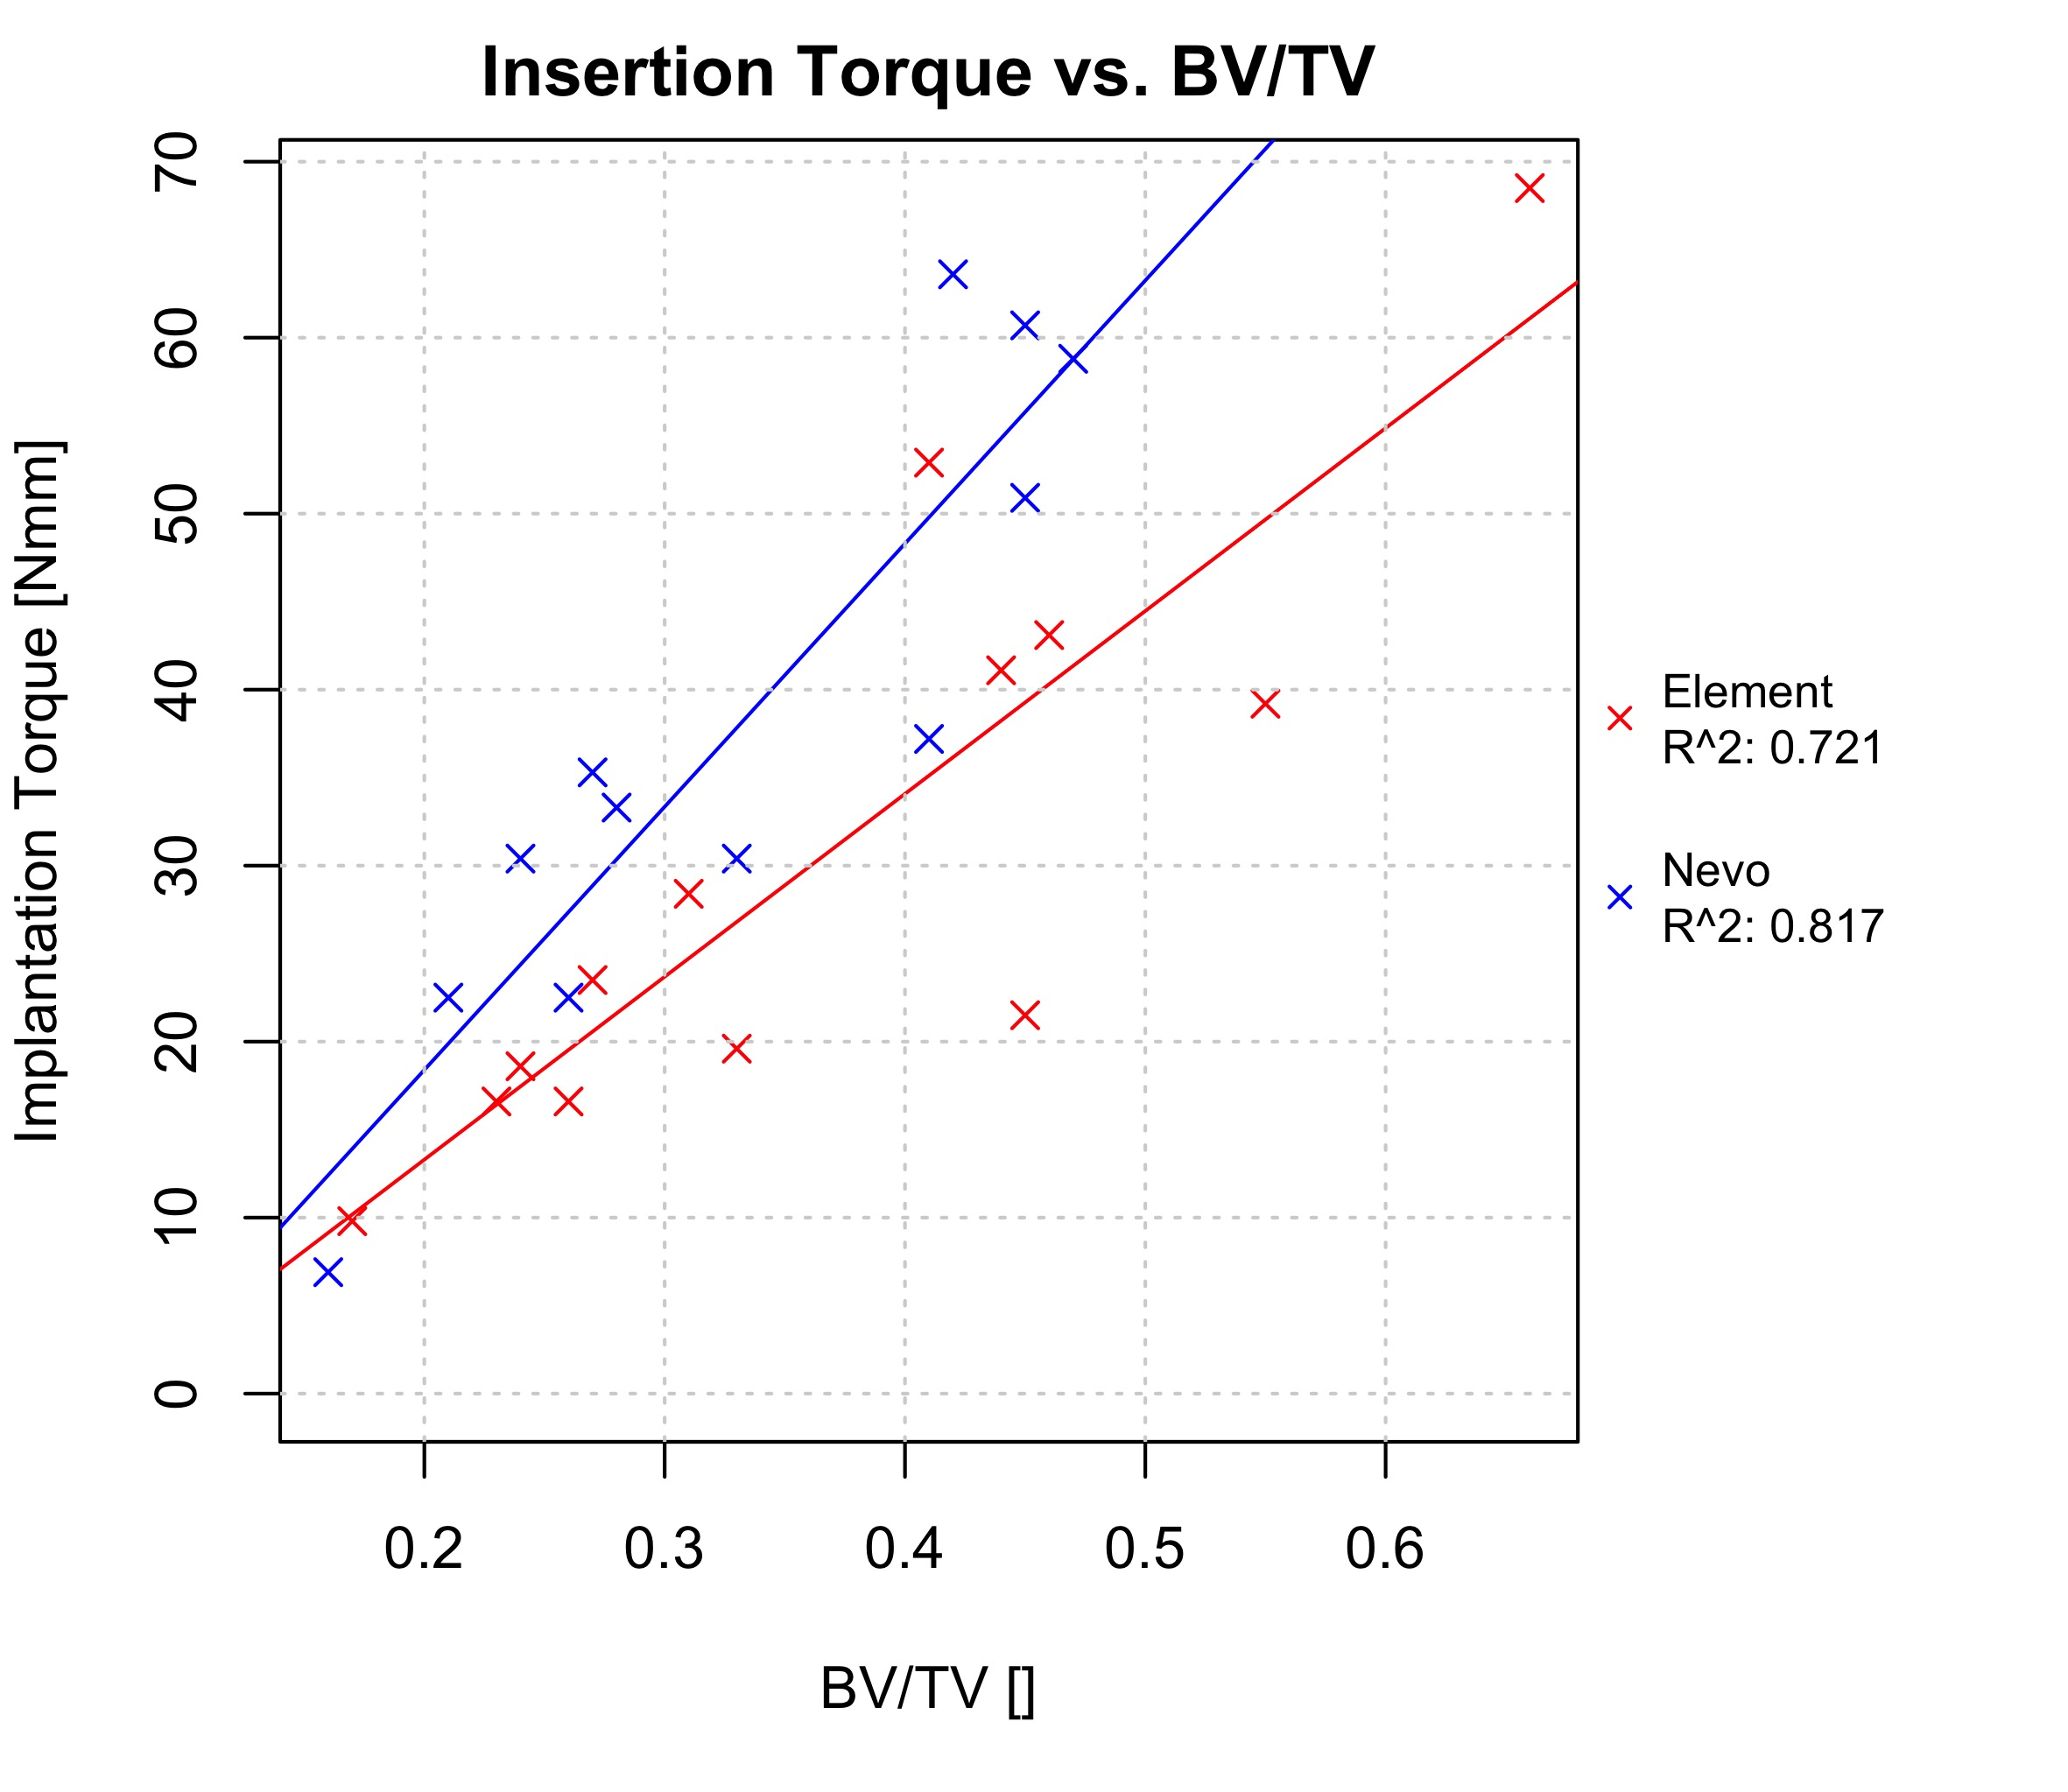
\includegraphics[width=0.49\textwidth]{figures/EXP_IT}}
\subfigure[]{\label{sublable2}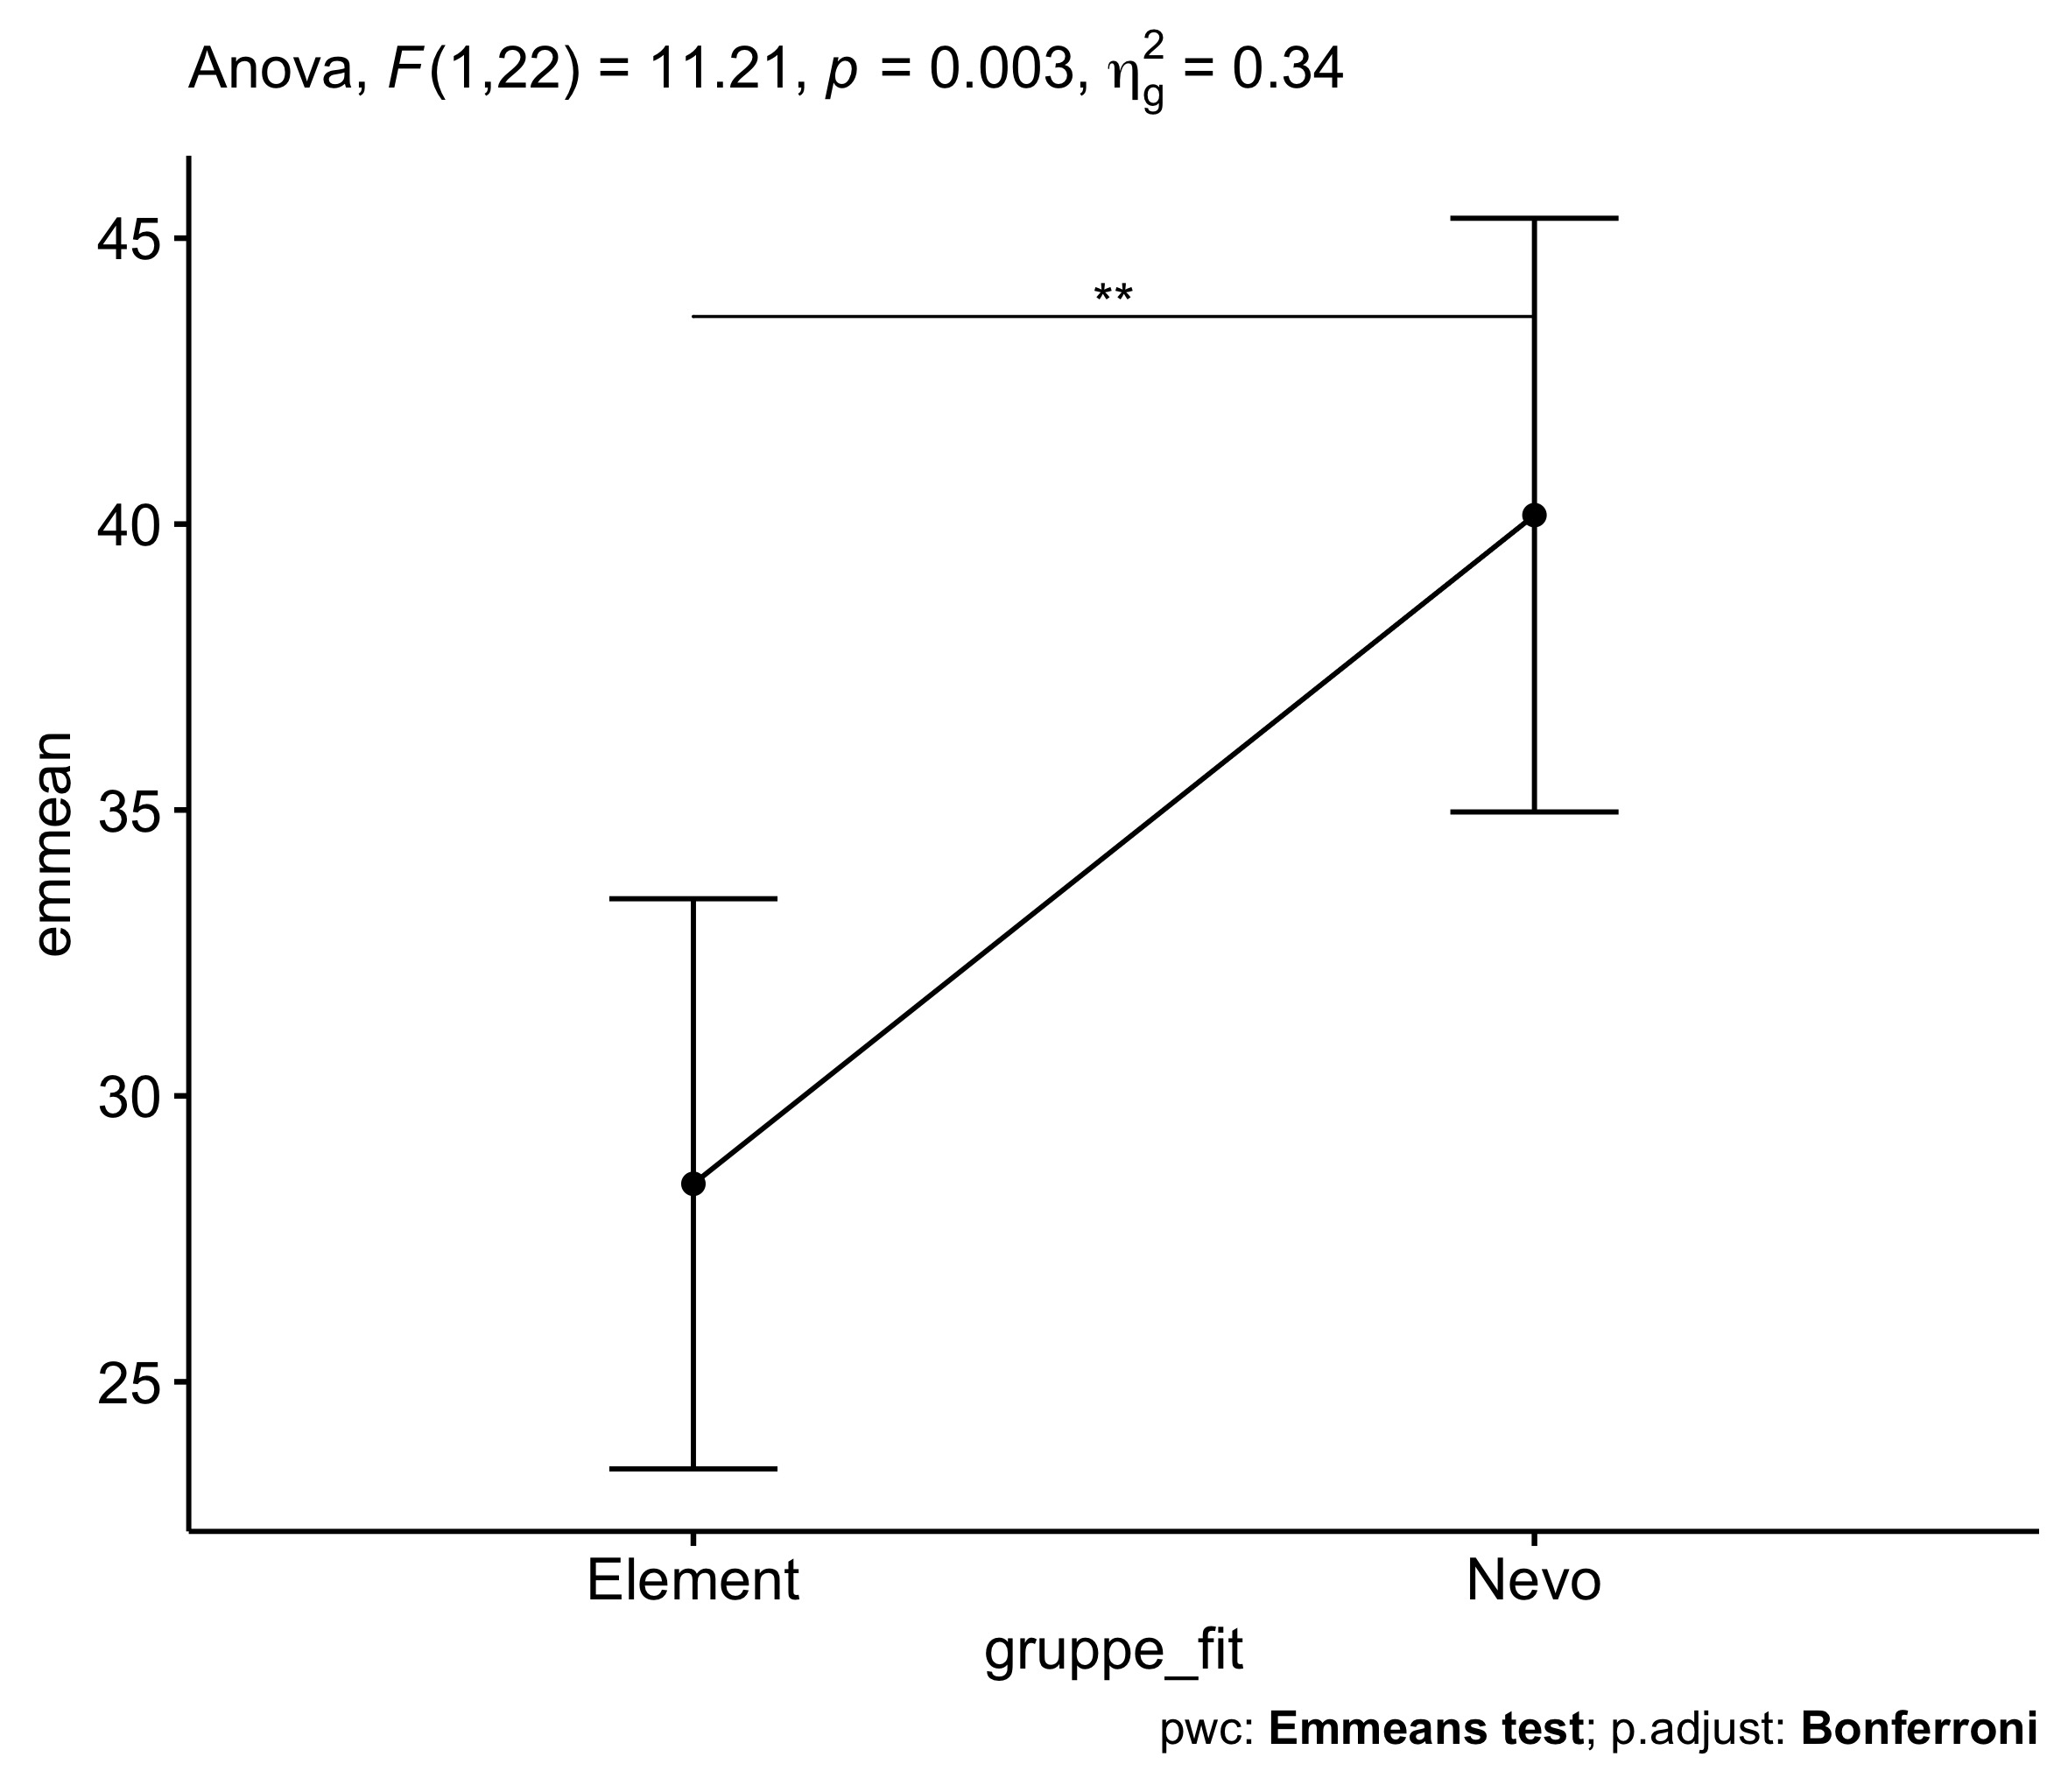
\includegraphics[width=0.49\textwidth]{figures/emmenas_IT}}
\captionof{figure}{(a): Insertion torque as a function of BV/TV with the individual linear regression model of each group. (b): Box plot of the estimated marginal means (emmeans or least square means) of each group after Bonferroni correction, controlled with BV/TV as covariate.}
\label{fig:RM_exp}
\end{figure}
%
\begin{table}[H]
\centering
\resizebox{300pt}{!}{%
\begin{tabular}{|l|c|c|c|c|c||c|}
	\hline
	& \multicolumn{5}{c||}{individual lin. regression} & eval. ANCOVA\\
	\hline 
	Group & $R^2$ & p-value & mean & RSE & CV & emmean $\pm$ StD\\
	\hline
	ELEMENT & 0.72 & 0.00015 & 30.72 & 9.028 & 0.56 & 28.46 $\pm$ ?\\
	\hline
	NEVO & 0.82 & 3.4e-5 & 37.71 & 7.49 & 0.46 & 40.16 $\pm$ ?\\
	\hline
\end{tabular}
}
\caption{Results for the linear regression (RSE: residual standard error, CV: coefficient of variation) of the experimentally evaluated implanting torque values. And the evaluation of the ANCOVA by the emmenas after Bonferroni correction.}
\label{tab:LGrm}
\end{table}
%
% G1 and G2 showed a significant linear relationship between implantation torque (IT) and BV/TV, where IT increases with increasing BV/TV. The linear relation in G3 is not significant but showed a tendency to the same behavior as the others.\\
% \\
The ANCOVA pointed out that the ultimate force was significantly related to the sample's BV$/$TV, F(1,22)=70.53, p$<$0.001.
Additionally, there was a significant difference between the groups on the insertion torque after controlling for the effect of the BV$/$TV with F(1,22)$=$11.21 and p$<$0.05.
% The ANCOVA pointed out that globally (over all groups) the insertion torque was significantly related to the sample's BV$/$TV, F(1,24)$=$41.5, p$<$0.001. Further more, there was a significant difference between the groups on the insertion torque after controlling for the effect of the BV$/$TV, F(2,24)$=$45.7, p$<$0.001.\\
% Through the post hoc analysis it could be observed that the emmeans of the insertion torque was significantly greater in G2 (169.0 Nmm) compared to G1 (110.0 Nmm) and G3 (52.3 Nmm) and G1 was greater than G3, p$<$0.001.
%
%
%
\subsection{Stiffness}
%
\begin{figure}[H]
\centering 
\subfigure[]{\label{sublable2}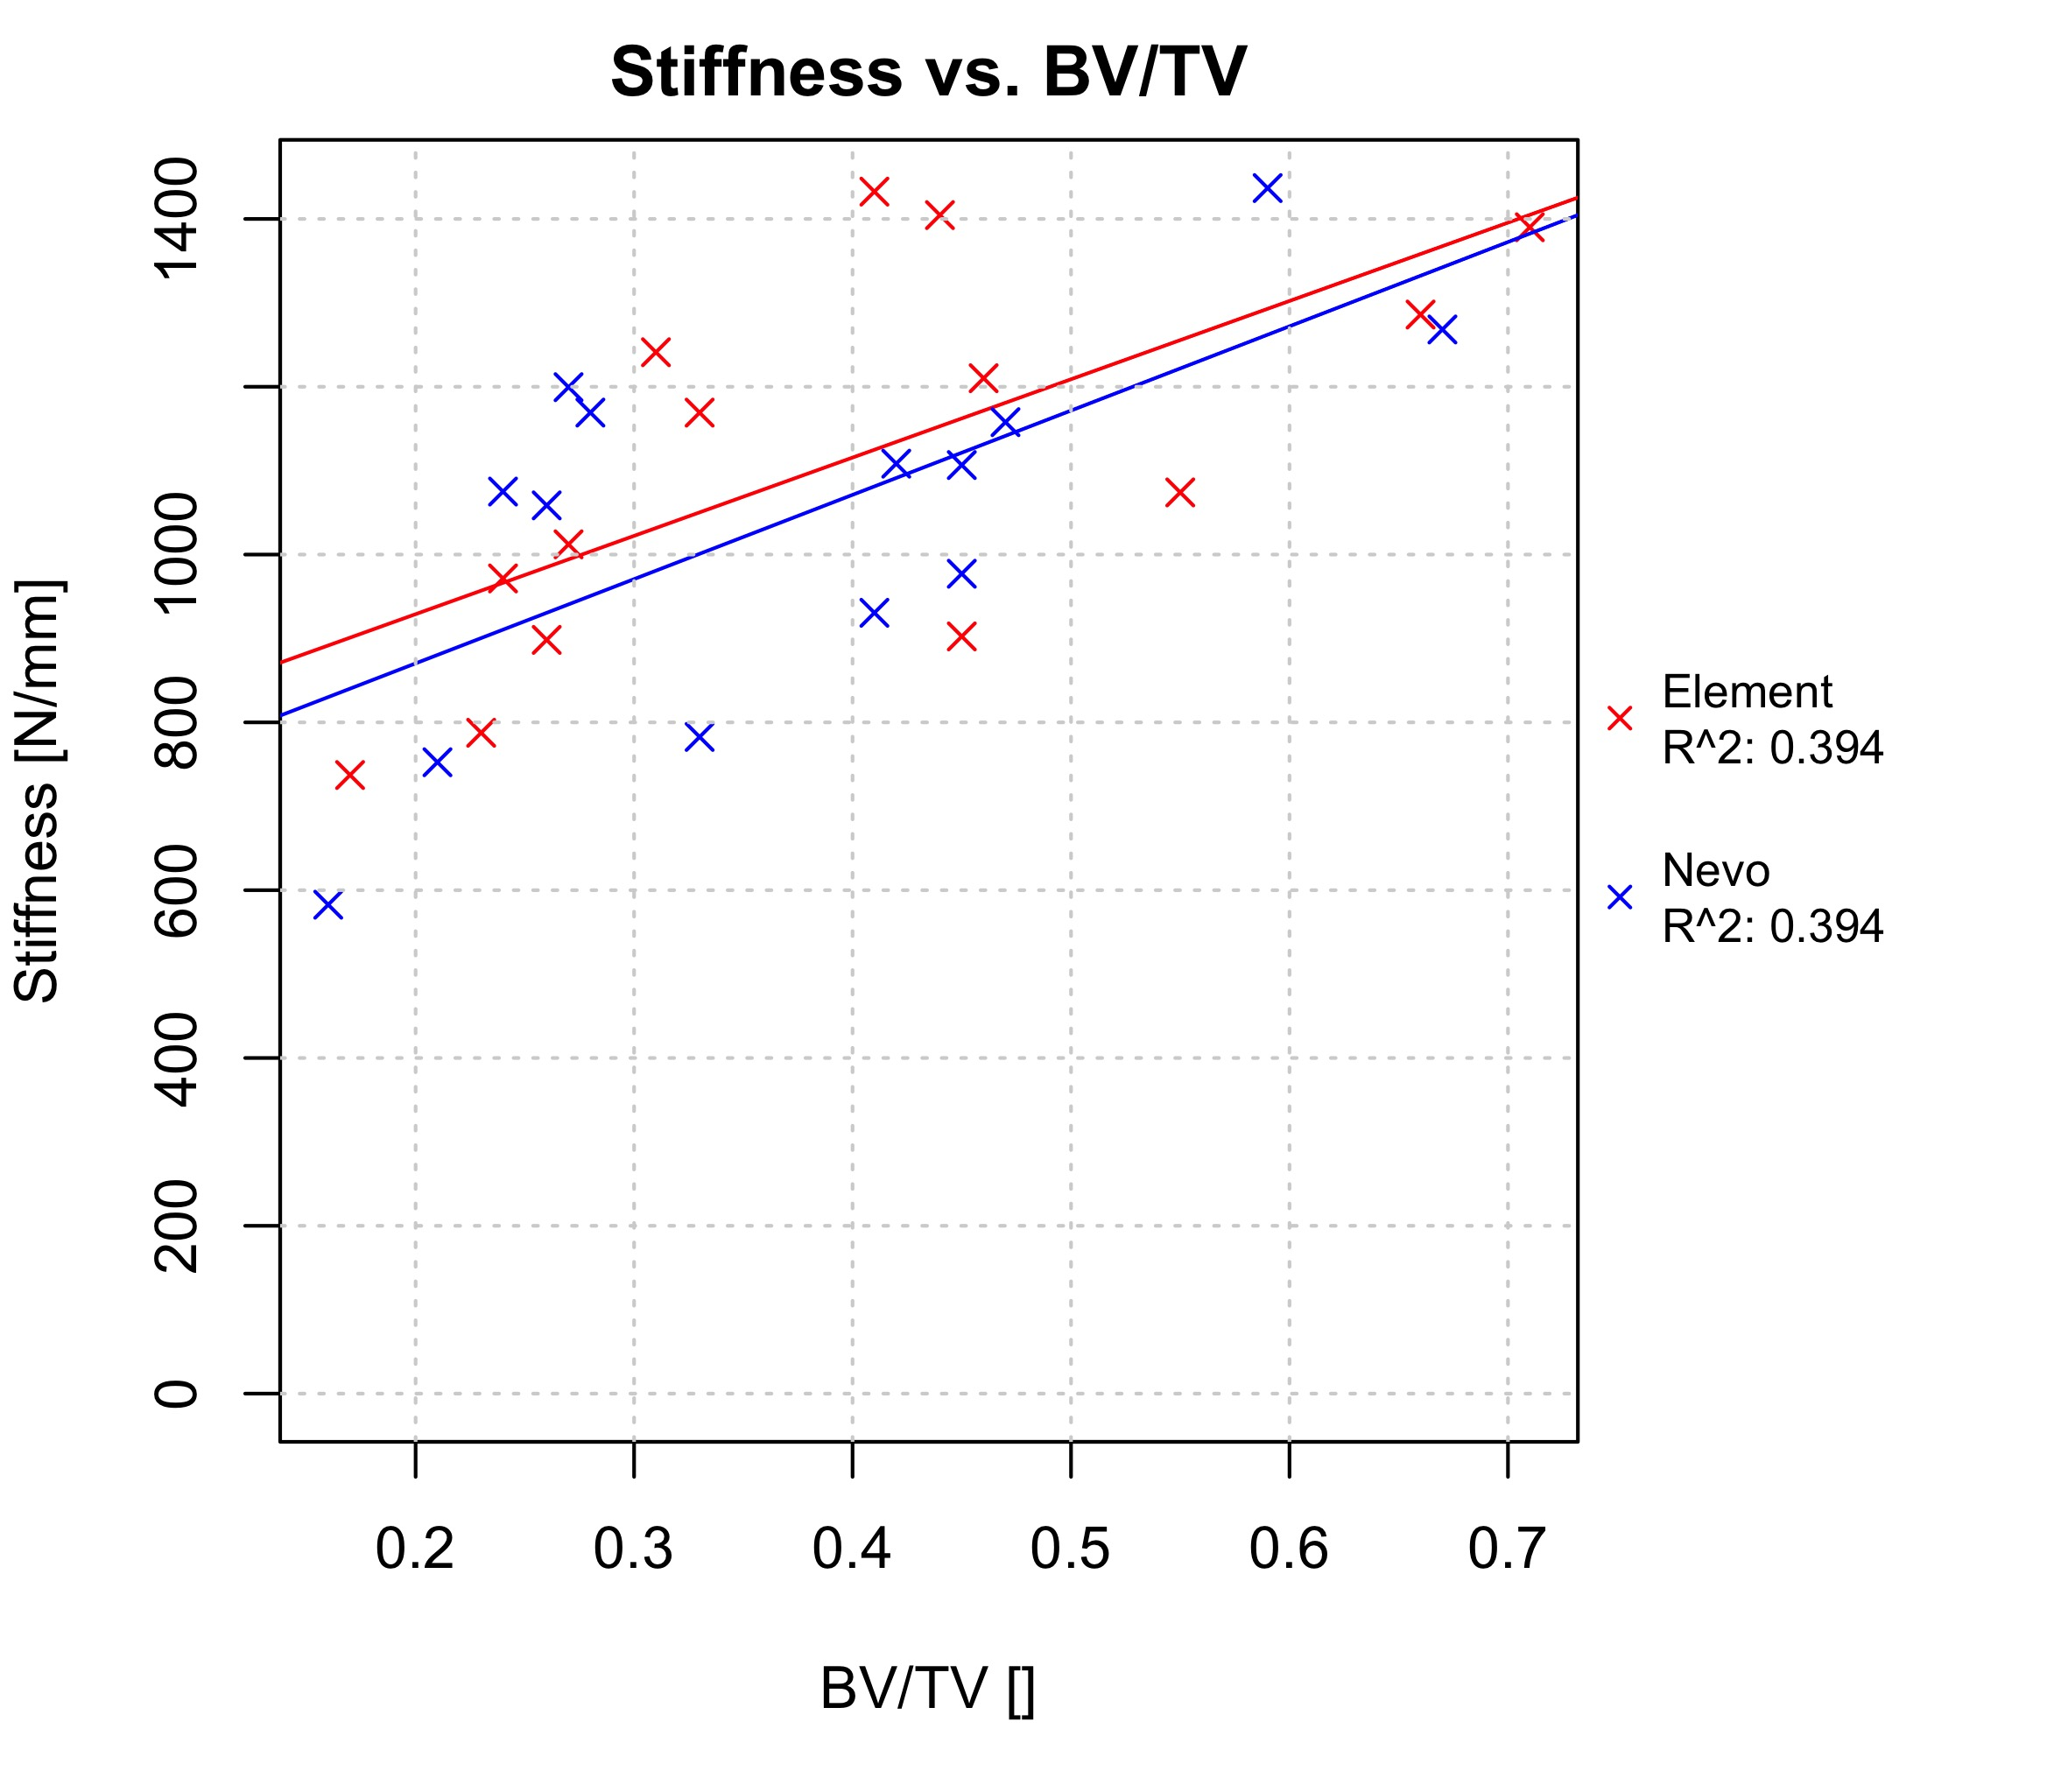
\includegraphics[width=0.49\textwidth]{figures/EXP_ST}}
\subfigure[]{\label{sublable2}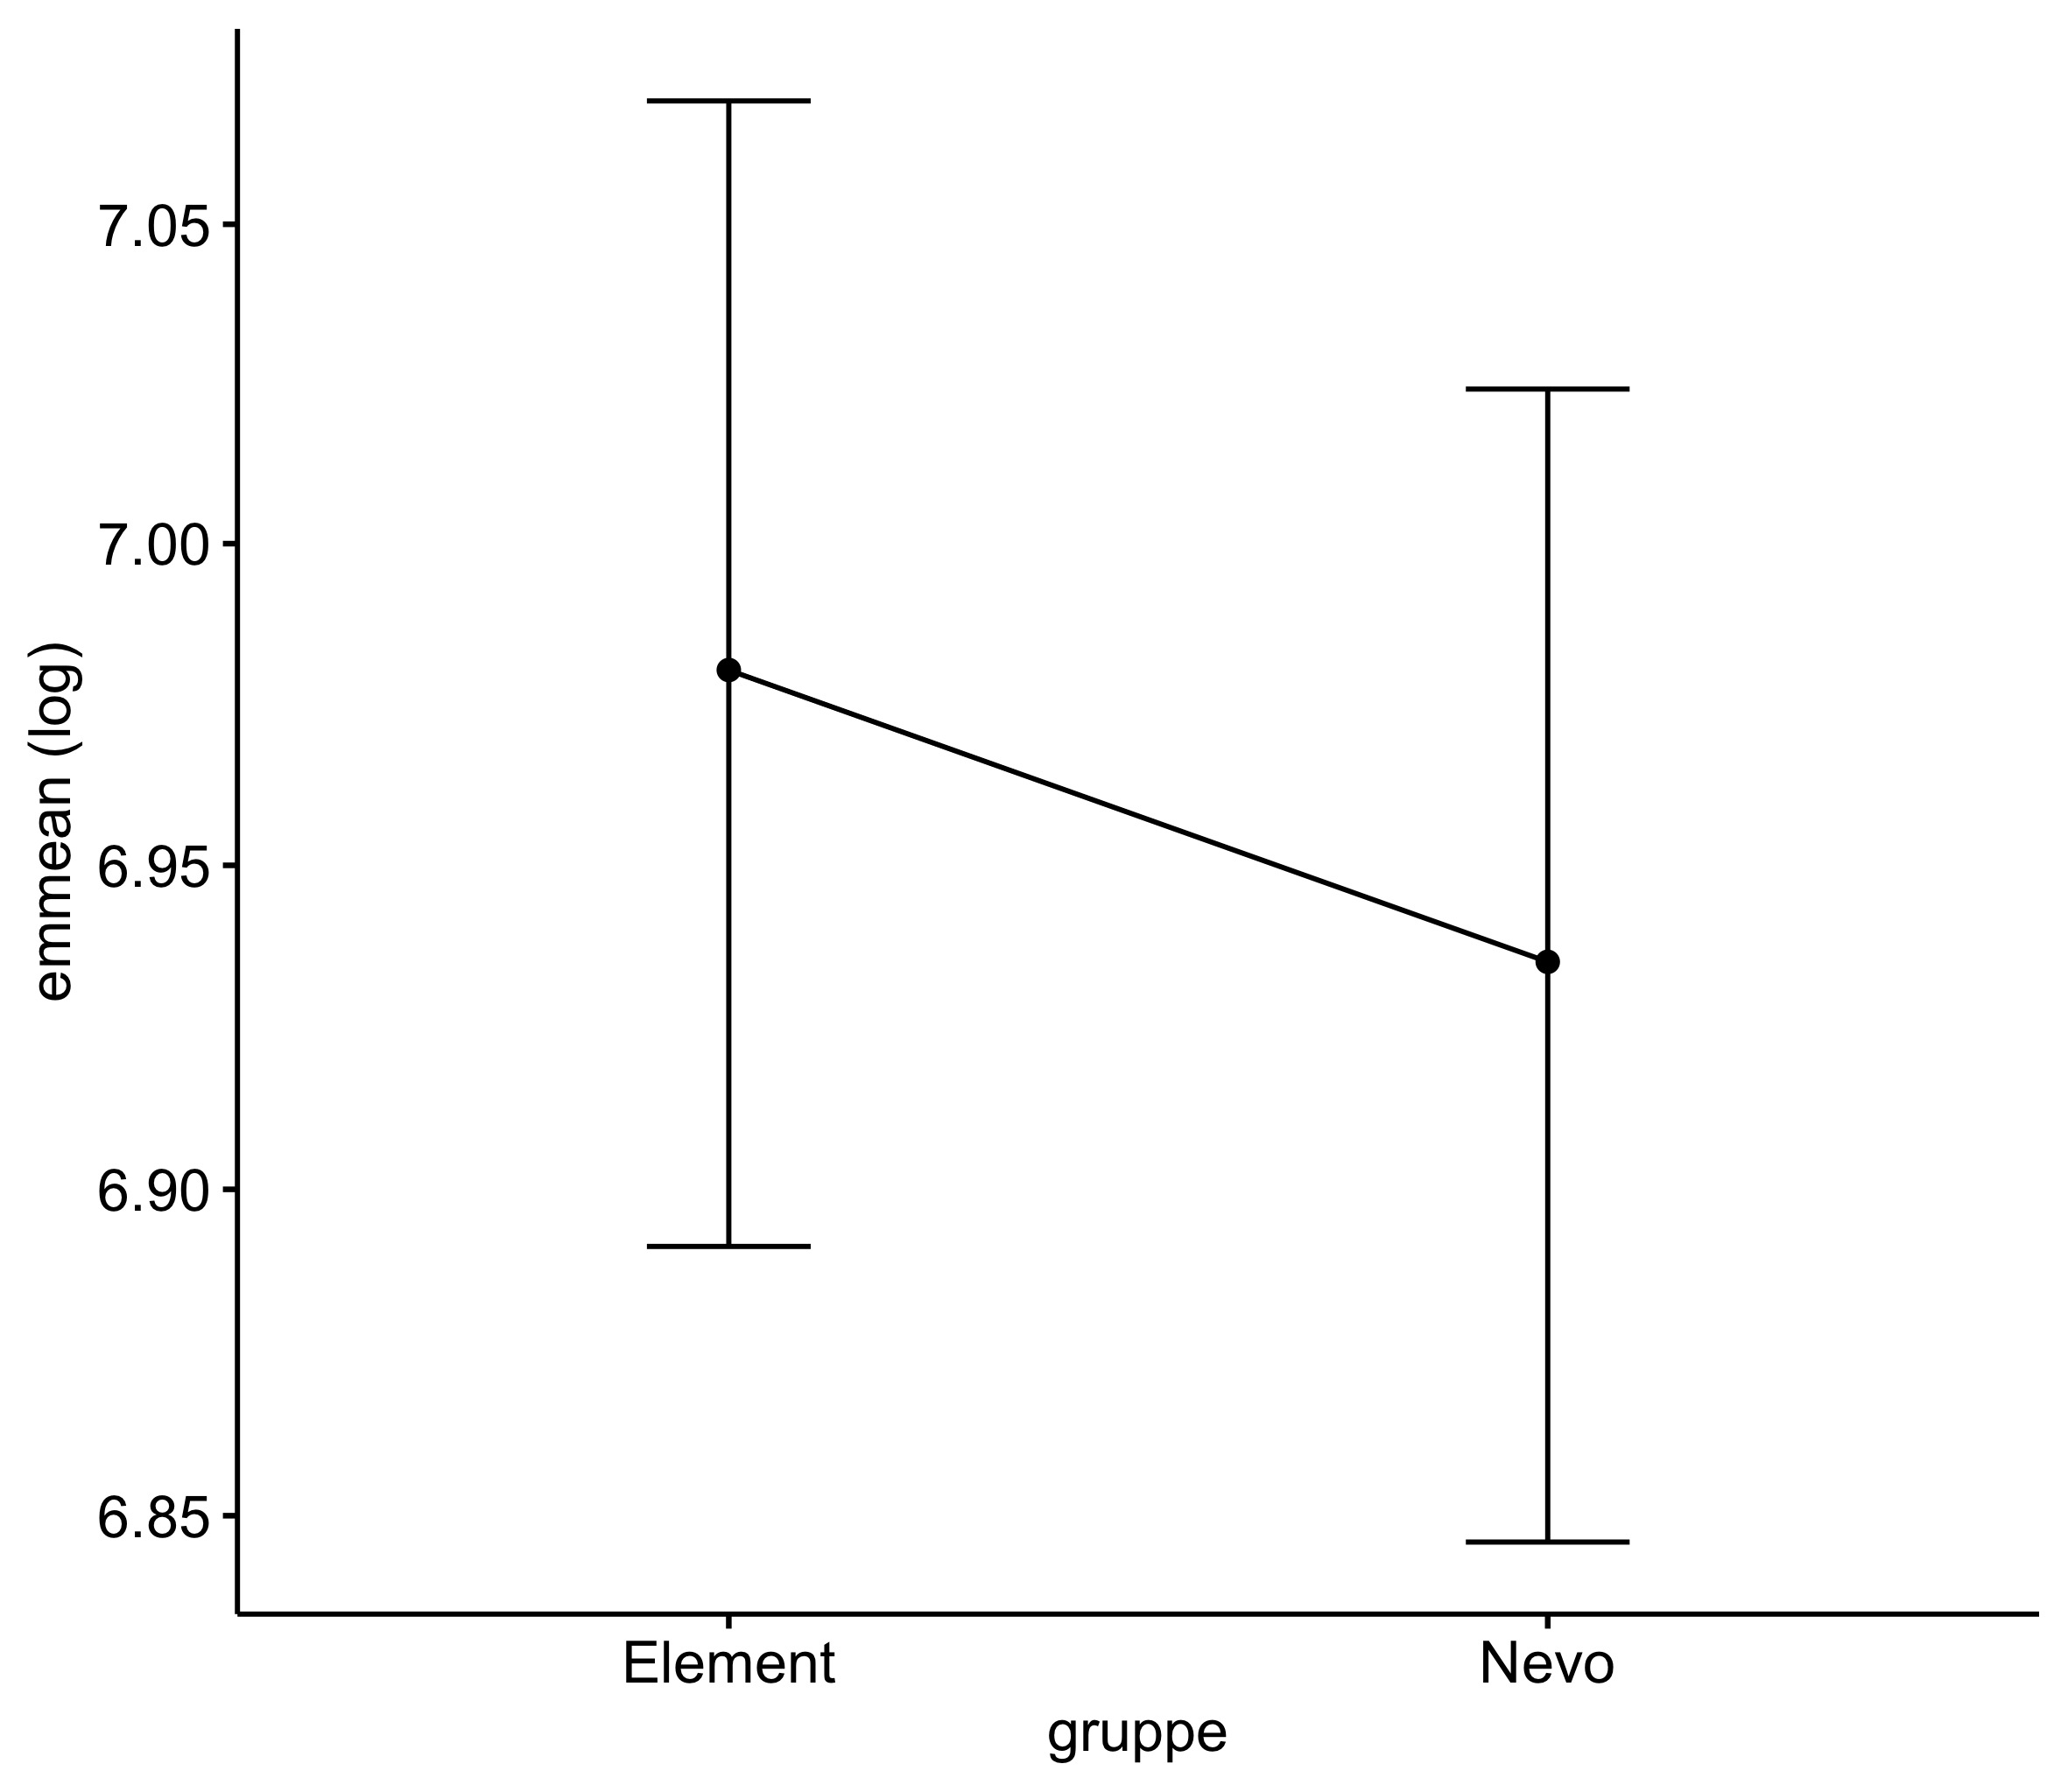
\includegraphics[width=0.49\textwidth]{figures/emmenas_ST}}
\captionof{figure}{(a): Insertion torque as a function of BV/TV with the individual linear regression model of each group. (b): Box plot of the estimated marginal means (emmeans or least square means) of each group after Bonferroni correction, controlled with BV/TV as covariate.}
\label{fig:RM_exp}
\end{figure}
%
\begin{table}[H]
\centering
\resizebox{300pt}{!}{%
\begin{tabular}{|l|c|c|c|c|c||c|}
	\hline
	& \multicolumn{5}{c||}{individual lin. regression} & eval. ANCOVA\\
	\hline 
	Group & $R^2$ & p-value & mean & RSE & CV & emmean $\pm$ StD\\
	\hline
	ELEMENT & 0.39 & 9.60e-3 & 1108.36 & 179.5 & 0.21 & 1098.42 $\pm$ ?\\
	\hline
	NEVO & 0.39 & 9.66e-3 & 1043.27 & 174.1 & 0.21 & 1053.23 $\pm$ ?\\
	\hline
\end{tabular}
}
	\caption{Results for the linear regression (RSE: residual standard error, CV: coefficient of variation) of the experimentally evaluated stiffness values. And the evaluation of the ANCOVA by the emmenas after Bonferroni correction and controlling for BV/TV.}
\label{tab:LGrm}
\end{table}
%
% G1 and G2 showed a significant linear relationship between implantation torque (IT) and BV/TV, where IT increases with increasing BV/TV. The linear relation in G3 is not significant but showed a tendency to the same behavior as the others.\\
% \\
The ANCOVA pointed out that the stiffness was significantly related to the sample's BV$/$TV, F(1,22)=70.53, p$<$0.001.
However, there was no significant difference between the groups on the ultimate force after controlling for the effect of the BV$/$TV, F(1,25)$=$0.50, p$>$0.05.
% The ANCOVA pointed out that globally (over all groups) the insertion torque was significantly related to the sample's BV$/$TV, F(1,24)$=$41.5, p$<$0.001. Further more, there was a significant difference between the groups on the insertion torque after controlling for the effect of the BV$/$TV, F(2,24)$=$45.7, p$<$0.001.\\
% Through the post hoc analysis it could be observed that the emmeans of the insertion torque was significantly greater in G2 (169.0 Nmm) compared to G1 (110.0 Nmm) and G3 (52.3 Nmm) and G1 was greater than G3, p$<$0.001.
%
%
%
\subsection{Ultimate Force}
%
\begin{figure}[H]
\centering 
\subfigure[]{\label{sublable2}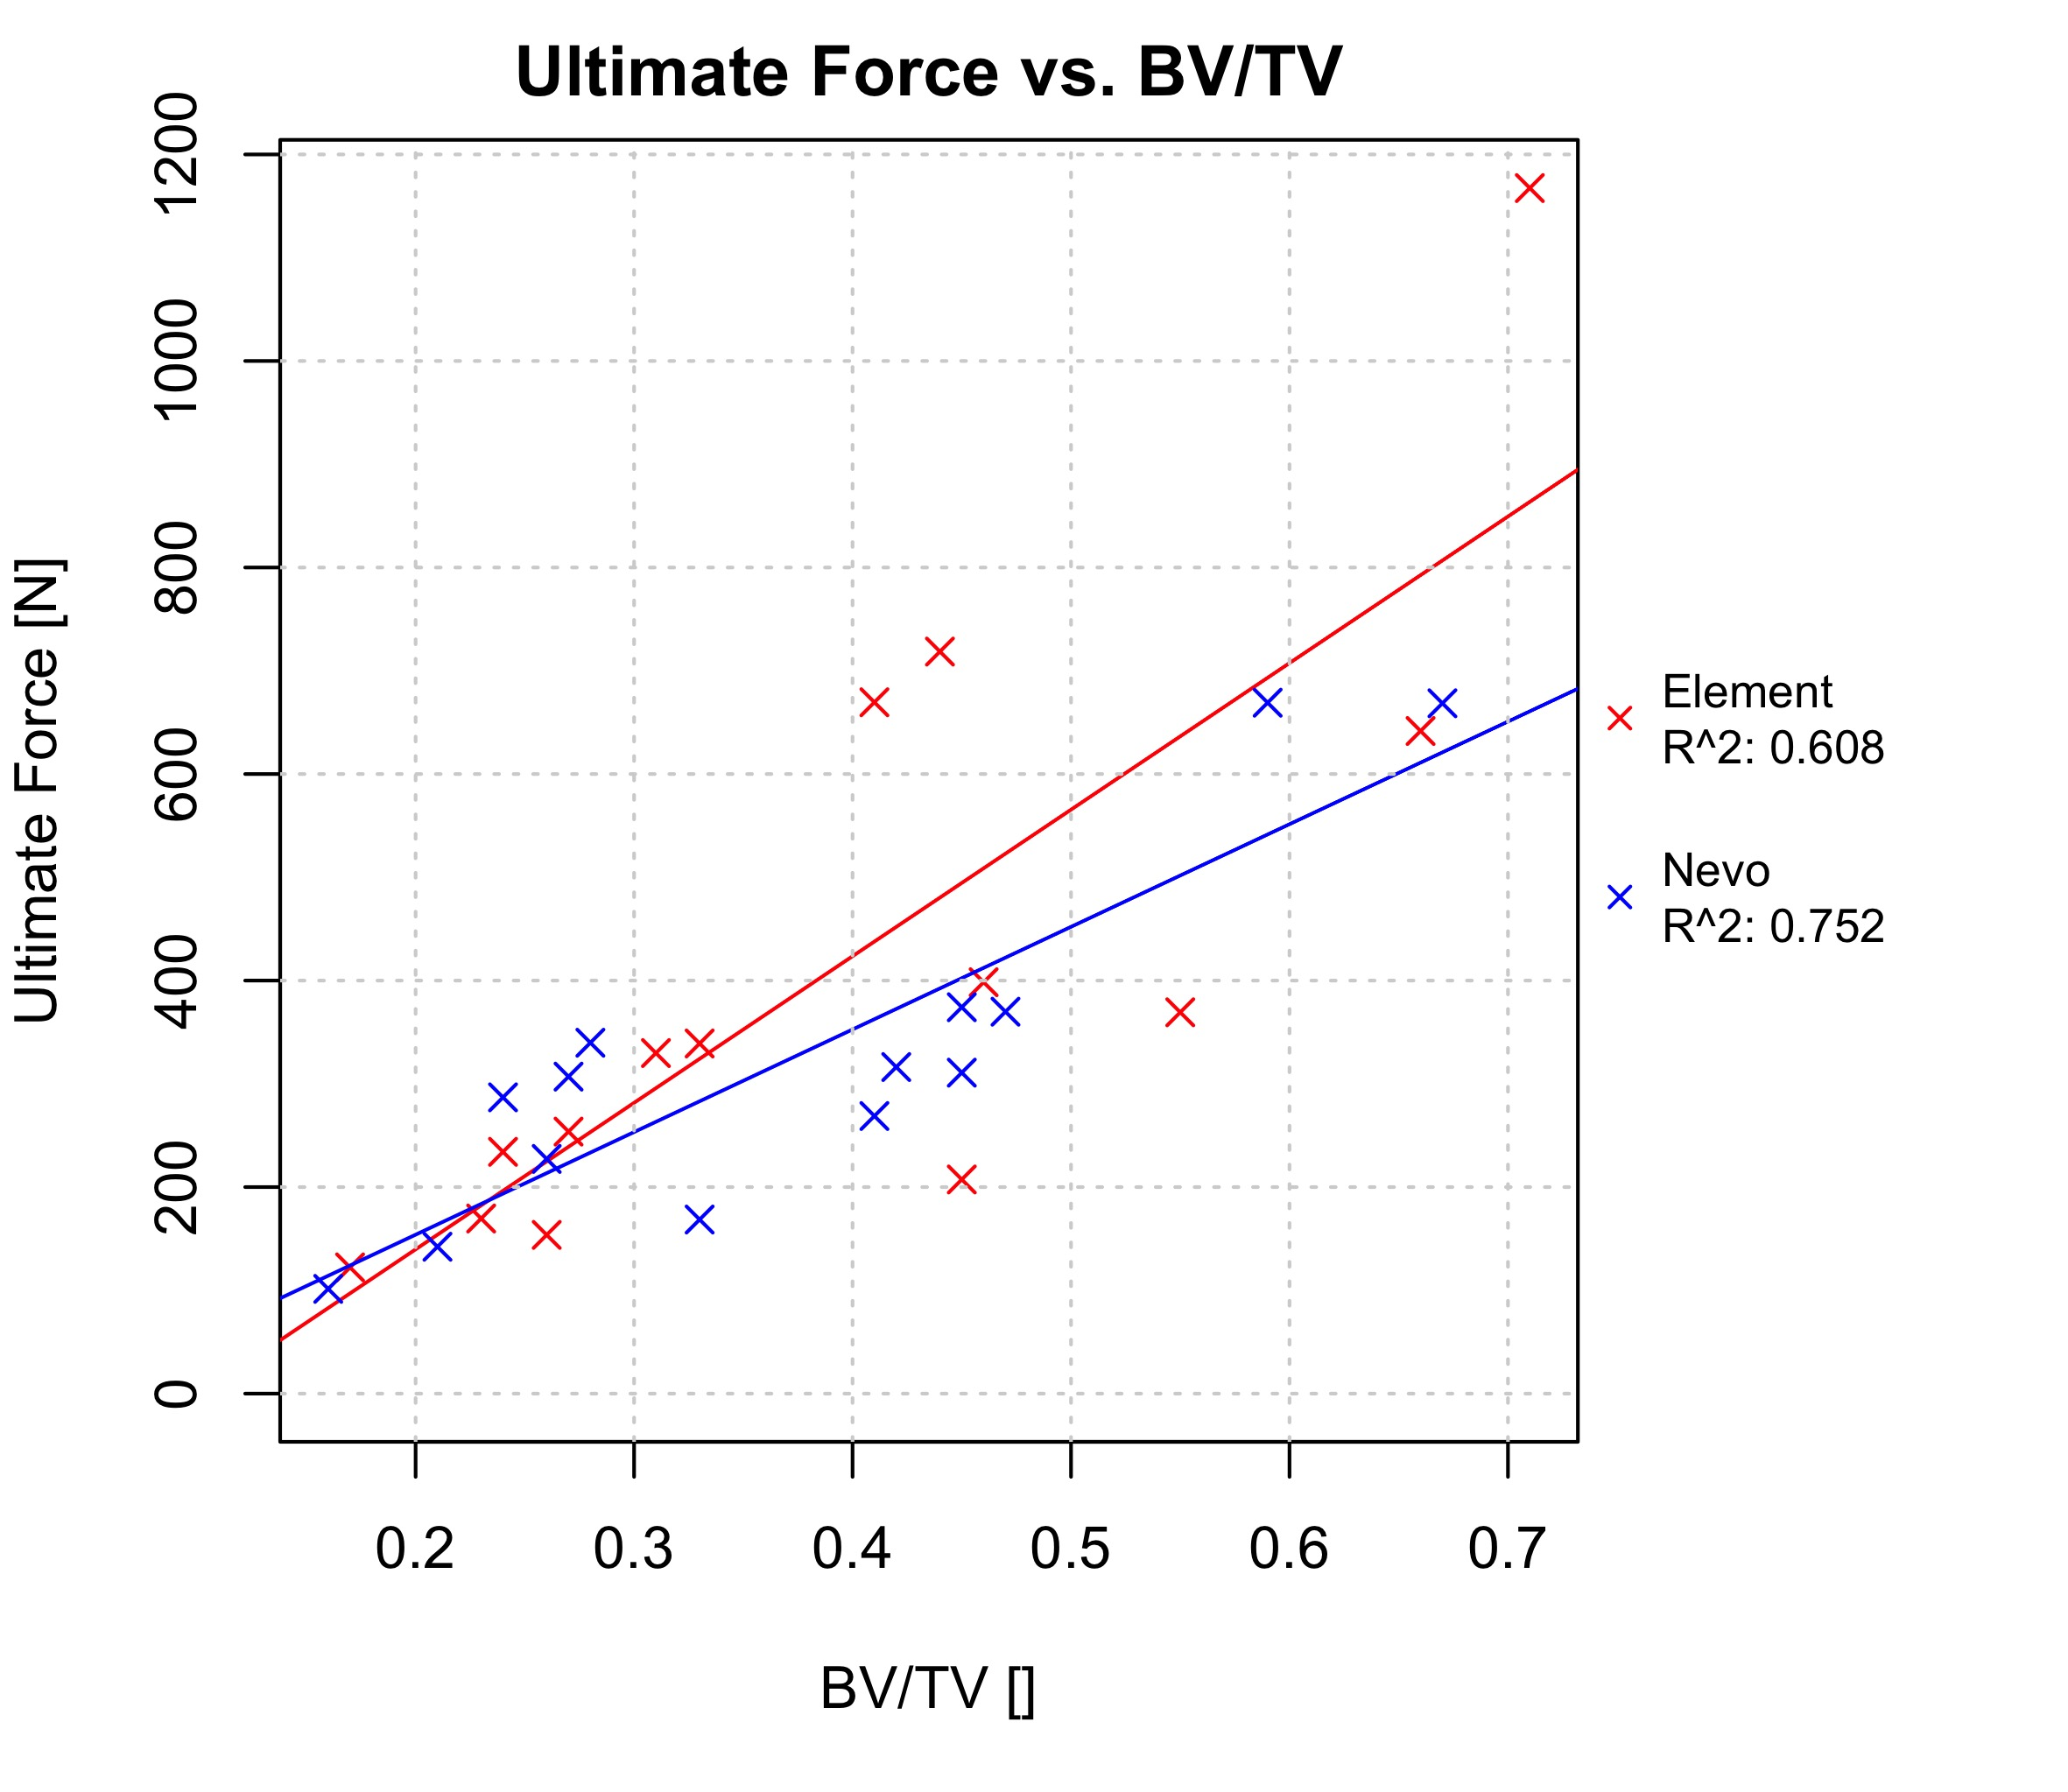
\includegraphics[width=0.49\textwidth]{figures/EXP_UF}}
\subfigure[]{\label{sublable2}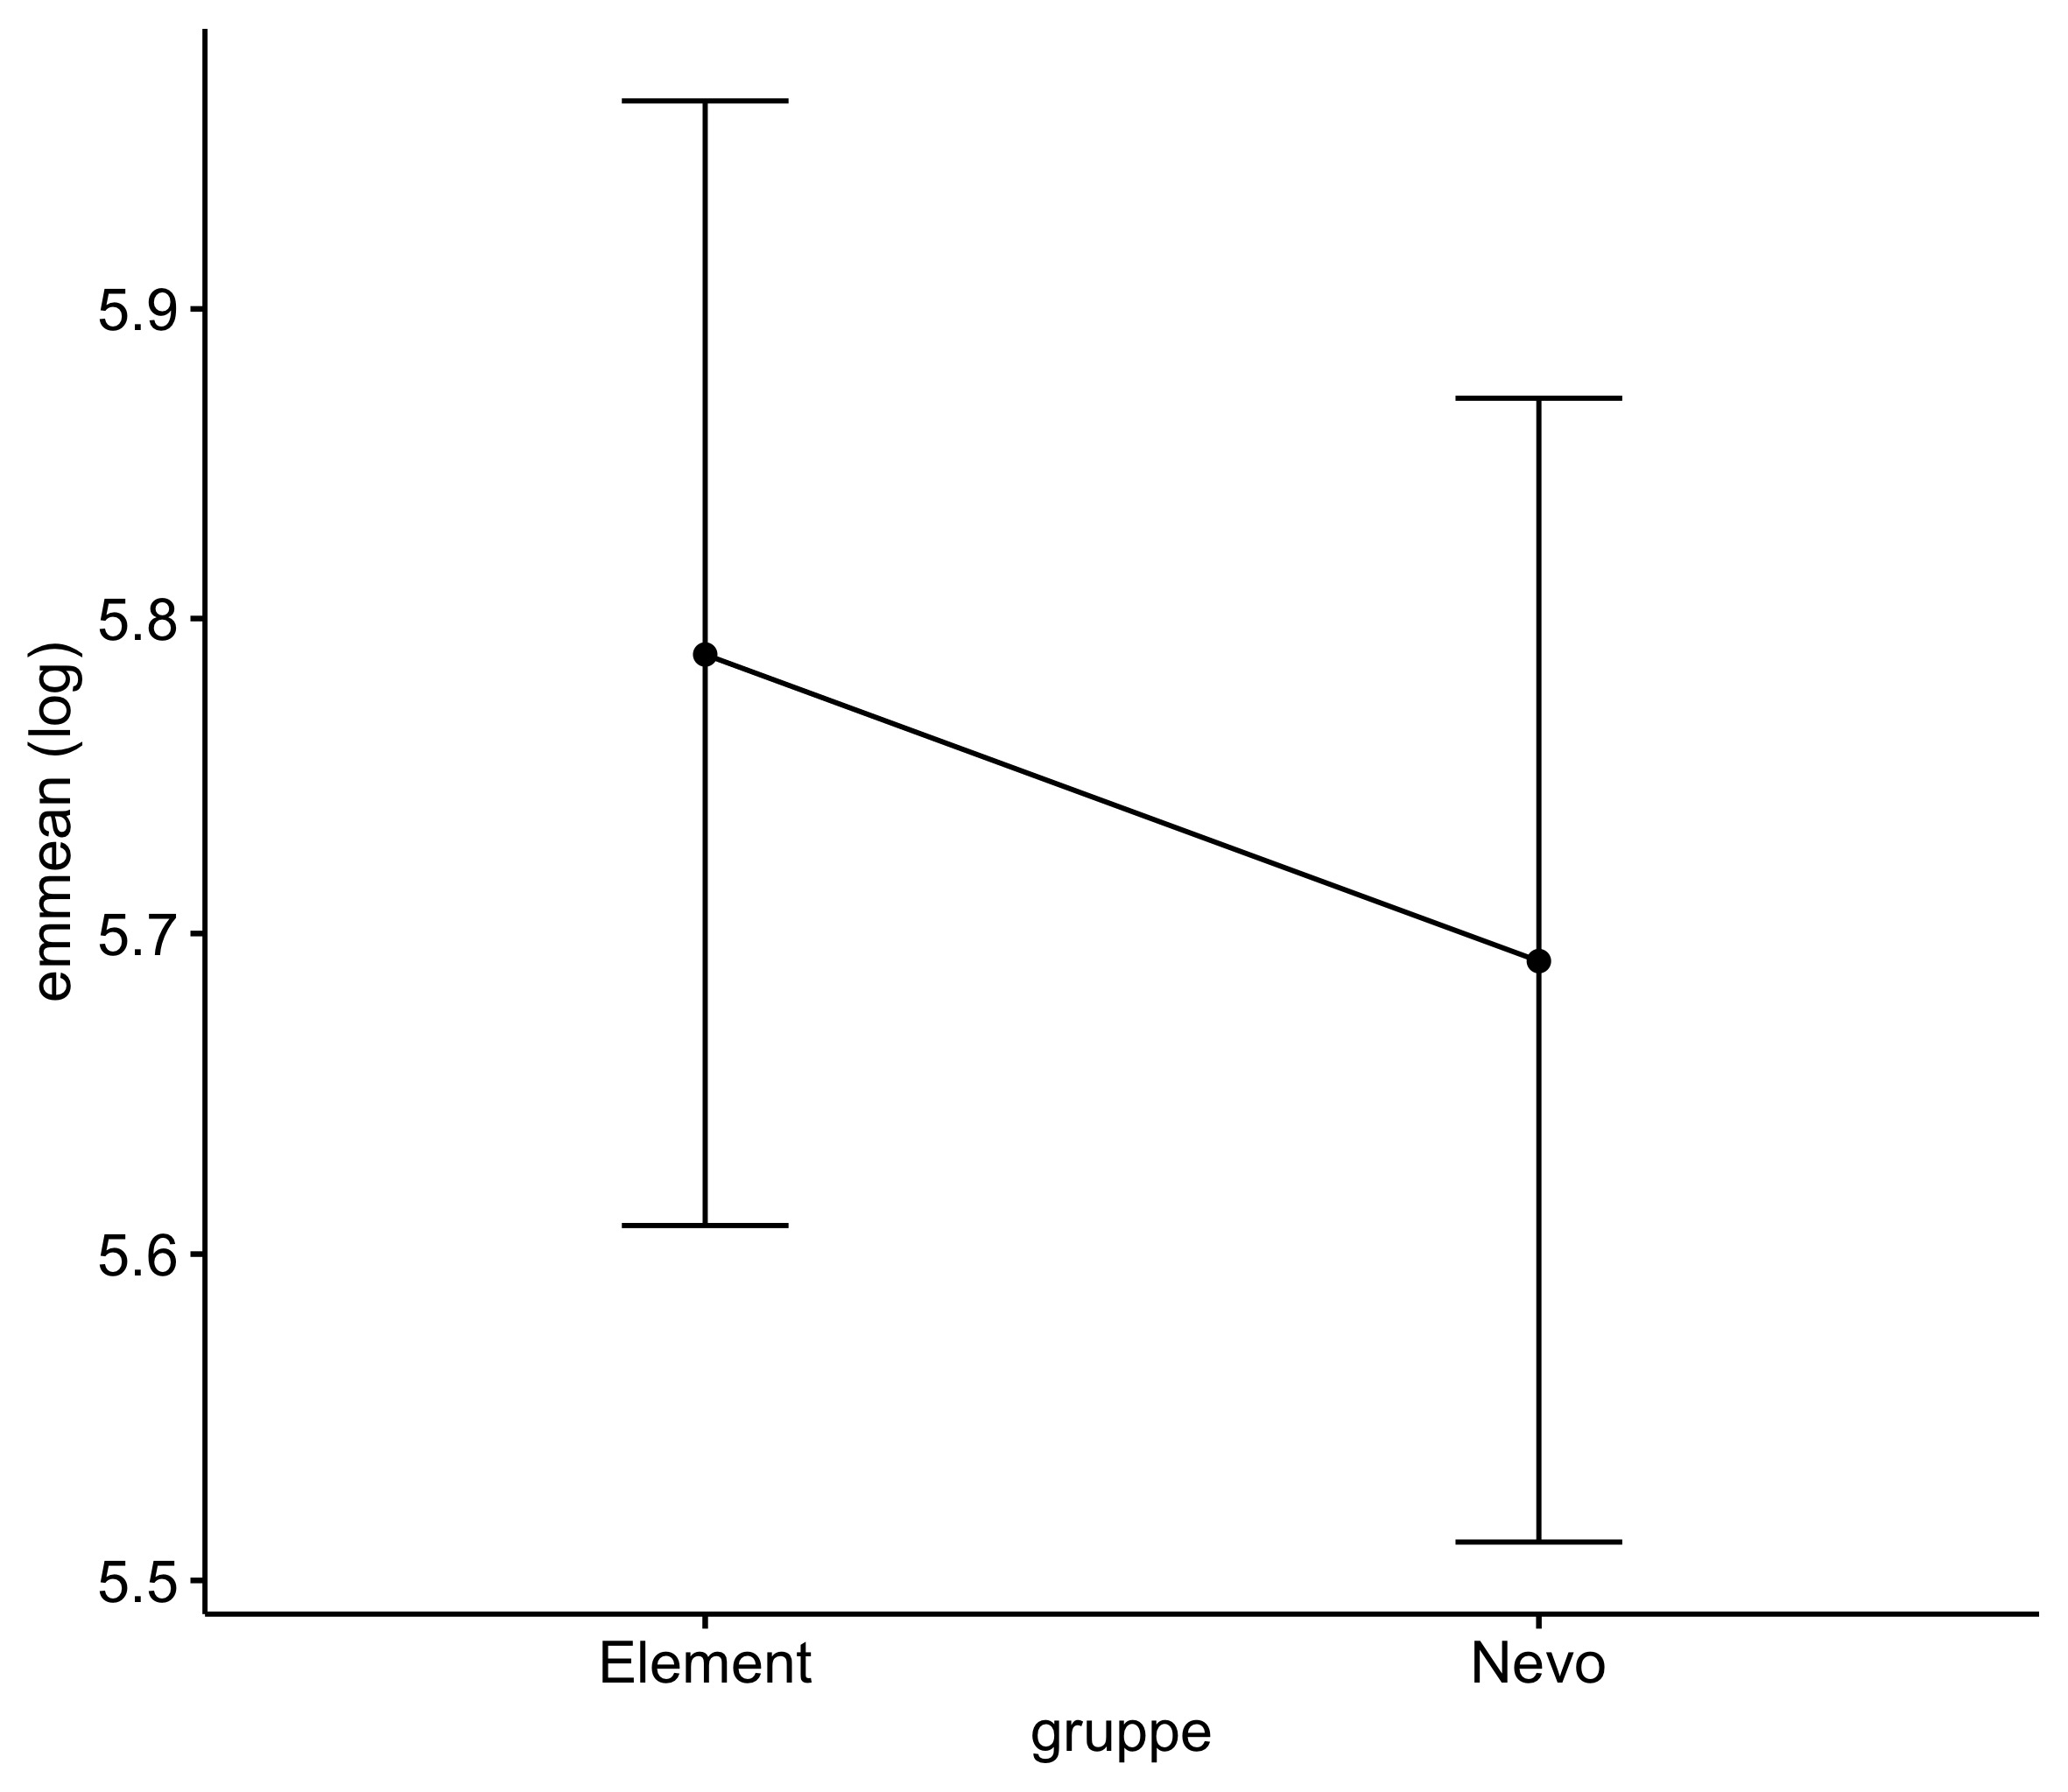
\includegraphics[width=0.49\textwidth]{figures/emmenas_UF}}
\captionof{figure}{(a): Ultimate force as a function of BV/TV with the individual linear regression model of each group. (b): Box plot of the estimated marginal means (emmeans or least square means) of each group after Bonferroni correction, controlled with BV/TV as the covariate.}
\label{fig:UF_exp}
\end{figure}
%
\begin{table}[H]
\centering
\resizebox{300pt}{!}{%
\begin{tabular}{|l|c|c|c|c|c||c|}
	\hline
	& \multicolumn{5}{c||}{individual lin. regression} & eval. ANCOVA\\
	\hline 
	Group & $R^2$ & p-value & mean & RSE & CV & emmean $\pm$ StD\\
	\hline
	ELEMENT & 0.61 & 6.13e-4 & 412.45 & 182.7 & 0.71 & 399.81 $\pm$ ?\\
	\hline
	NEVO & 0.75 & 3.65e-5 & 325.06 & 83.33 & 0.51 & 337.69 $\pm$ ?\\
	\hline
\end{tabular}
}
\caption{Results for the linear regression (RSE: residual standard error, CV: coefficient of variation) of the experimentally evaluated ultimate force values. And the evaluation of the ANCOVA by the emmeans after Bonferroni correction.}
\label{tab:LGuf}
\end{table}
%
% G1 and G3 showed a significant linear relationship between implantation ultimate force (UF) and BV/TV, where UF increases with increasing BV/TV. The linear relation in G2 is not significant but showed a strong tendency to the same behaviour as the others.\\
% \\
The ANCOVA pointed out that the ultimate force was significantly related to the sample's BV$/$TV, F(1,25)=47.51, p$<$0.001.
However, there was no significant difference between the groups on the ultimate force after controlling for the effect of the BV$/$TV, F(1,25)$=$1.33, p$>$0.05.
% The ANCOVA pointed out that globally (over all groups) the ultimate force was significantly related to the sample's BV$/$TV, F(1,24)$=$100.5, p$<$0.001. Further more, there was a significant difference between the groups on the ultimate force after controlling for the effect of the BV$/$TV, F(2,24)$=$34.8, p$<$0.001.\\
% Through the post hoc analysis it could be observed that the emmeans of the ultimate force is not significantly greater in G1 (701.0N) compared to G2 (608.0N), p$>$0.05. The mean ultimate force was significantly lower in G3 (283N) compared to G2 and G1. p$<$0.001.
%
%
%
\newpage
%
%
%
\chapter{Discussion, limitations and conclusion}
%
%
%
\section{Discussion and Limitations}

% notes new report:
- Andere Belastungsart: vertikal nicht angewinkelt.
- Rotationssteiffigkeit: dort nicht se ein grosser Unterschied.
- Haben das Implantat nochmals geändert.

%
The statically evaluated experimental data shows, that under-drilling (G1: final drill $\O=$3.5mm, G2: final drill $\O=$2.8mm) does significantly increases the insertion torque, while no significant differences in ISQ, stiffness nor ultimate force could be detected. This means, that the here performed under-drilling, did not improve the objective primary stability of the SPI ELEMENT implant. \\
Furthermore, a significant reduction of the insertion torque, ISQ, stiffness and ultimate force was observed for a partial insertion of the implant (G3: insertion depth $=$ 6.5mm, which is 41$\%$ reduction with respect to the standard implantation depth of 11mm). The observed reductions were not identical for insertion torque (reduced by 52$\%$), ISQ (reduced by 28$\%$), stiffness (reduced by 17$\%$), ultimate force (reduced by 60$\%$). For BV/TV range of G3, ISQ showed no dependency on BV/TV as it would be expected. This could be explained by the nature of the ISQ measurement, which relies on the resonance frequency of the implant and its surrounding. It appears therefore that the geometrical difference of the insertion dominates the mechanical properties of the bone ISQ measurement. 

During the drilling procedure using the CNC drilling machine, it was easy to reach the desired depth. Nevertheless, during implantation it was very hard to control the depth, which of course might have a big influence on the primary stability parameters (for the vertical loading configuration). 

%
\begin{table}[H]
\centering
\begin{tabular}{|l|l|}
	\hline 
	\multicolumn{2}{|l|}{Hypothesis 1:}\\
	\multicolumn{2}{|l|}{Under-drilling will ...} \\
	\hline
	increase the insertion torque & \multicolumn{1}{c|}{TRUE} \\
	\hline
	increase the ISQ & \multicolumn{1}{c|}{FALSE}\\
	\hline
	does not effect the objective primary stability & \multicolumn{1}{c|}{TRUE} \\
	\hline
	\hline 
	\multicolumn{2}{|l|}{Hypothesis 2:}\\
	\multicolumn{2}{|l|}{Partial insertion will ...} \\
	\hline
	reduce the insertion torque & \multicolumn{1}{c|}{TRUE} \\
	\hline
	reduce the ISQ & \multicolumn{1}{c|}{TRUE}\\
	\hline
	reduce the objective primary stability & \multicolumn{1}{c|}{TRUE} \\
	\hline
\end{tabular}
\caption{Overview of results in relation to the working hypotheses.}
\label{tab:LGuf}
\end{table}
%
The simulated insertion torque showed similar values than the experiment. For the simulated stiffness and the ultimate force similar trends could be observed in the simulation as in the experiments. Never the less, the simulation tends to overestimate the values (stiffness and ultimate force) for low BV/TV samples and vice-versa for high BV/TV samples which can be seen in fig. \ref{fig:UF_simvsexp}. Furthermore, the vertical test setting could lead to uncertainties, caused by the drilled hole which is 0.4mm deeper than the actual implantation depth or due to tilting of the partially inserted implant in G3. The former could lead to an increased stability in the experiment if the implant is implanted slightly deeper than the 11mm and the latter could decrease the stability in the experiment if the implant is tilted during the test. Both situations were not be captured by the simulation. At last, the simulation is not able to fully include densification or bone compaction which has a higher effect on high BV/TV samples than for low BV/TV samples.
%
\begin{figure}[H]
\centering 
\subfigure[]{\label{sublable2}\includegraphics[width=0.49\textwidth]{figures_old/Simulation/RM_SIMvsEXP_02G1G2G3}}
\subfigure[]{\label{sublable2}\includegraphics[width=0.49\textwidth]{figures_old/Simulation/ST_SIMvsEXP_02G1G2G3}}
\subfigure[]{\label{sublable2}\includegraphics[width=0.49\textwidth]{figures_old/Simulation/UF_SIMvsEXP_02G1G2G3}}
\captionof{figure}{(a): Simulated insertion torque in relation to the insertion torque measured during the experiment. (b) Simulated stiffness in relation to the stiffness measured during the experiment.(c): Simulated ultimate force in relation to the ulitmate force measured during the experiment.}
\label{fig:UF_simvsexp}
\end{figure}
%
%
%
\newpage
%
\section{Conclusions}
%
Through the experiments it could be shown that under-drilling did not improve the primary stability of the SPI ELEMENT implant. Furthermore, there was no significant difference visible for the ISQ between G1 and G2 as hypothesised. It seems that the ISQ changes only weakly with increasing BV/TV and had no dependency for partially inserted implants.

The partially inserted implants showed markedly decreased values for all measured parameters (insertion torque, ISQ and objective primary stability).

The FE-simulations showed similar tendencies as the experiments, especially for the simulated insertion torque. To make more specific statements, more simulations are needed.

%The structural differences between the samples can lead to variances in the simulated results as it can be seen in the experiments. It seems that simulating only the min and max BV/TV samples is not sufficient for a proper evaluation by the FE-simulation.


%According to the ISQ measurements, for the group G3, there is no visible relationship with BV/TV and it is clearly different from Group G1 and Group G2. It leads to the conclusion that measuring ISQ values on not completely inserted implants is not very meaningful. 
\newpage
%
\chapter{Additional Task: New Implant design}
%
A new implant design with a adapted drilling protocol was numerically tested and compared with the simulation of the results of the G1 group (See fig. \ref{fig:New_Imp}). For the comparison the same three bone samples were used as for the simulations of the G1 group (See tab. \ref{tab:StudyDesign}). The simulation of the new implant type was performed as described before.
%
\begin{figure}[H]
\centering 
\label{sublable2}\includegraphics[width=0.49\textwidth]{figures_old/newImp/New_Imp.png}
\captionof{figure}{The compared implants with their corresponding profile of the osteotomie (left: SPI ELEMENT, right: new design).}
\label{fig:New_Imp}
\end{figure}
%
\section{Results}
%
The new implant design seams to have the tendency to have higer implant torque, stiffness and ultimate force as the SPI ELEMENT implant (See fig. \ref{fig:newVSold}). The differences are more clear in the higher BV/TV range and less in the lower BV/TV range, especially for stiffness and ultimate force.
%
\begin{figure}[H]
\centering 
\subfigure[]{\label{sublable2}\includegraphics[width=0.49\textwidth]{figures_old/newImp/rm_oldVSnew}}
\subfigure[]{\label{sublable2}\includegraphics[width=0.49\textwidth]{figures_old/newImp/st_oldVSnew}}
\subfigure[]{\label{sublable2}\includegraphics[width=0.49\textwidth]{figures_old/newImp/uf_oldVSnew}}
\captionof{figure}{Comparison of the existing SPI ELEMENT implant with a new implant desgin. (a): Simulated insertion torque. (b) Simulated stiffness.(c): Simulated ultimate force.}
\label{fig:newVSold}
\end{figure}
%
%
\begin{figure}[H]
\centering 
\subfigure[]{\label{sublable2}\includegraphics[width=0.49\textwidth]{figures_old/newImp/T3_12_RMZ_Imp}}
\subfigure[]{\label{sublable2}\includegraphics[width=0.49\textwidth]{figures_old/newImp/T4_05_RMZ_Imp}}
\subfigure[]{\label{sublable2}\includegraphics[width=0.49\textwidth]{figures_old/newImp/T4_09_RMZ_Imp}}
\captionof{figure}{Direct comparison of the insertion torque for the existing SPI ELEMENT implant with the new implant design for bone sample T3\_12 (a), T4\_05 (b) and T4\_09 (c).}
\label{fig:RFdirect}
\end{figure}
%
\begin{figure}[H]
\centering 
\subfigure[]{\label{sublable2}\includegraphics[width=0.49\textwidth]{figures_old/newImp/T3_12_RFZ_Imp}}
\subfigure[]{\label{sublable2}\includegraphics[width=0.49\textwidth]{figures_old/newImp/T4_05_RFZ_Imp}}
\subfigure[]{\label{sublable2}\includegraphics[width=0.49\textwidth]{figures_old/newImp/T4_09_RFZ_Imp}}
\captionof{figure}{Direct comparison of the stiffness and ultimate force for the existing SPI ELEMENT implant with the new implant design for bone sample T3\_12 (a), T4\_05 (b) and T4\_09 (c).}
\label{fig:UFdirect}
\end{figure}
%
\section{Discussion and Conclusion}
%
The simulation of the new implant with the adapted drilling protocol showed a tendency to higher insertion torque and better primary implant stability as the existing implant design (SPI ELEMENT). For a statistical evaluation more simulations are needed.
%
\chapter{Simulation of all Samples}
%
\begin{figure}[H]
\centering 
\label{sublable2}\includegraphics[width=1\textwidth]{figures_old/intern/RM_SIMvsEXP_02G1allallG2allG3all}
\captionof{figure}{Insertion torque}
\label{fig:New_Imp}
\end{figure}
%
\begin{figure}[H]
\centering 
\label{sublable2}\includegraphics[width=1\textwidth]{figures_old/intern/Log_ST_SIMvsEXP_02G1allallG2allG3all}
\captionof{figure}{LOG-LOG plot of Stiffness}
\label{fig:New_Imp}
\end{figure}
%
\begin{figure}[H]
\centering 
\label{sublable2}\includegraphics[width=1\textwidth]{figures_old/intern/Log_ST_SIMvsEXP_02allGroups}
\captionof{figure}{LOG-LOG plot of Stiffness}
\label{fig:New_Imp}
\end{figure}
%
\begin{figure}[H]
\centering 
\label{sublable2}\includegraphics[width=1\textwidth]{figures_old/intern/Log_UF_SIMvsEXP_02G1allallG2allG3all}
\captionof{figure}{LOG-LOG plot of ultimate force}
\label{fig:New_Imp}
\end{figure}
%
\begin{figure}[H]
\centering 
\label{sublable2}\includegraphics[width=1\textwidth]{figures_old/intern/Log_UF_SIMvsEXP_02allGroups}
\captionof{figure}{LOG-LOG plot of ultimate force}
\label{fig:New_Imp}
\end{figure}
%
\begin{figure}[H]
\centering 
\label{sublable2}\includegraphics[width=1\textwidth]{figures_old/intern/BDIdev_SIMvsBVTV_02G1allallG2allG3all}
\captionof{figure}{Deviatoric BDI}
\label{fig:New_Imp}
\end{figure}
%
\begin{figure}[H]
\centering 
\label{sublable2}\includegraphics[width=1\textwidth]{figures_old/intern/BDIhyd_SIMvsBVTV_02G1allallG2allG3all}
\captionof{figure}{Hydrostatic BDI}
\label{fig:New_Imp}
\end{figure}
%
\appendix
\chapter{Appendix}
\newpage
\section*{Appendix A}
\begin{table}[H]
\begin{tabular}{l|l|l|l|l|l|l|l}
Prot. & Sample & $\#$ & BV/TV {[}-{]} & IT {[}Nmm{]} & Stiff. {[}N/mm{]} & UF {[}N{]} & ISQ {[}-{]} \\ \hline
G1       & T3\_01 & 18 & 0.32          & 143.94            & 23203.39             & 876.08                 & 69          \\
G1       & T3\_08 & 6 & 0.27          & 102.71            & 19484.48             & 729.62                 & 65          \\
G1       & T3\_11 & 3 & 0.22          & 73.72             & 11319.39             & 433.23                 & 61          \\
G1       & T3\_12 & 7 & 0.27          & 121.27            & 10011.02             & 568.79                 & 61.5        \\
G1       & T4\_01 & 4 & 0.25          & 129.75            & 16302.53             & 616.48                 & 64.5        \\
G1       & T4\_02 & 17 & 0.32          & 105.96            & 18576.89             & 561.43                 & 63          \\
G1       & T4\_05 & 1 & 0.16          & 49.38             & 3843.84              & 190.77                 & 51          \\
G1       & T4\_07 & 15 & 0.28          & 83.36             & 27621.11             & 689.26                 & 61.5        \\
G1       & T4\_09 & 21 & 0.38          & 193.50            & 43607.98             & 1306.78                & 69          \\
G1       & T4\_10 & 20 & 0.36          & 125.97            & 29780.10             & 1017.57                & 67          \\
G1       & T5\_01 & 2 & 0.21          & 83.63             & 6473.56              & 384.72                 & 62          \\
G1       & T5\_02 & 16 & 0.29          & 116.86            & 23997.21             & 829.86                 & 65.5        \\
G1       & T5\_06 & 5 & 0.26          & 82.20             & 10073.35             & 596.92                 & 62.5        \\
G1       & T5\_11 & 19 & 0.35          & 125.15            & 19119.80             & 1048.05                & 66.5        \\
G2       & T3\_03 & 11 & 0.25          & 162.74            & 21816.34             & 655.83                 & 65.5        \\
G2       & T3\_04 & 14 & 0.27          & 149.52            & 15081.85             & 481.38                 & 62.5        \\
G2       & T3\_09 & 8 & 0.16          & 107.96            & 5332.09              & 272.88                 & 60          \\
G2       & T3\_10 & 9 & 0.21          & 112.52            & 10444.89             & 293.49                 & 57          \\
G2       & T4\_06 & 13 & 0.27          & 198.62            & 13949.68             & 487.64                 & 64          \\
G2       & T4\_08 & 10 & 0.22          & 134.49            & 14444.72             & 379.21                 & 64          \\
G2       & T5\_07 & 12 & 0.26          & 169.27            & 9813.84              & 431.97                 & 59          \\
G3       & T3\_02 & 28 & 0.38          & 78.13             & 10839.85             & 537.97                 & 45          \\
G3       & T3\_07 & 22 & 0.28          & 45.78             & 3542.62              & 244.97                 & 44          \\
G3       & T4\_03 & 25 & 0.32          & 88.90             & 8481.32              & 492.02                 & 51.5        \\
G3       & T5\_03 & 23 & 0.30          & 79.06             & 12850.83             & 432.48                 & 51.5        \\
G3       & T5\_08 & 24 & 0.31          & 60.27             & 7261.70              & 431.63                 & 47.5        \\
G3       & T5\_09 & 26 & 0.35          & 87.45             & 11077.54             & 537.78                 & 52          \\
G3       & T5\_10 & 27 & 0.36          & 74.12             & 12508.04             & 526.74                 & 46         
\end{tabular}
\caption{Experiment - Sample list with Prot.(Protocol); Sample; Numbering; BV/TV; IT (Implantation Torque); Stiff. (Stiffness); UF (Ultimate Force); ISQ.}
\label{tab:TabSamples}
\end{table}
%
\newpage
\begin{table}[H]
    \begin{tabular}{l|l|l|l|l|l|l}

        Port.    & Sample & $\#$  & BV/TV [-] & IT [Nmm] & Stiff. [N/mm] & UF [N] \\ \hline
        G1       & T4\_05  & 1  & 0.16      & 49.9     & 3386.6        & 509.4  \\ 
        G1       & T3\_12  & 7  & 0.27      & 86.3     & 2637.0        & 909.2  \\ 
        G1       & T4\_09  & 21 & 0.38      & 165.9    & 4245.7        & 1178.5 \\ 
        G2       & T3\_09  & 8  & 0.16      & 81.7     & 1729.1        & 526.1  \\ 
        G2       & T3\_04  & 14 & 0.27      & 166.7    & 2807.5        & 541.0  \\ 
        G3       & T3\_07  & 22 & 0.28      & 51.5     & 2011.7        & 504.7  \\ 
        G3       & T3\_02  & 28 & 0.38      & 90.7     & 3192.9        & 605.4  \\ 
        new Imp. & T4\_05  & 1  & 0.16      & 70.5     & 3328.8        & 550.3  \\ 
        new Imp. & T3\_12  & 7  & 0.27      & 18.7     & 8967.9        & 1146.5 \\ 
        new Imp. & T4\_09  & 21 & 0.38      & 198.7    & 12500.7       & 1670.5 \\

    \end{tabular}
		\caption{Simulation - Sample list with Prot.(Protocol); Sample; Numbering; BV/TV; IT (Implantation Torque); Stiff. (Stiffness); UF (Ultimate Force); ISQ.}
		\label{tab:TabSamples_sim}
\end{table}

\newpage
%
%
%

%

%
%%%%%%%%%%%%%%%%%%%%%%%%%%%%%%%%%%%%%%%%%%%%%%%%%%%%%%%%%%%%%%%%%%%%%
\backmatter
\bibliographystyle{apalike}
\bibliography{biblio}

%%%%%%%%%%%%%%%%%%%%%%%%%%%%%%%%%%%%%%%%%%%%%%%%%%%%%%%%%%%%%%%%%%%%% 
%%%%%%%%%%%%%%%%%%%%%%%%%%%%%%%%%%%%%%%%%%%%%%%%%%%%%%%%%%%%%%%%%%%%% 
\end{document}
%%%%%%%%%%%%%%%%%%%%%%%%%%%%%%%%%%%%%%%%%%%%%%%%%%%%%%%%%%%%%%%%%%%%%
%%%%%%%%%%%%%%%%%%%%%%%%%%%%%%%%%%%%%%%%%%%%%%%%%%%%%%%%%%%%%%%%%%%%%
%%%%%%%%%%%%%%%%%%%%%%%%%%%%%%%%%%%%%%%%%%%%%%%%%%%%%%%%%%%%%%%%%%%%%
